%% ==============================================================================
%% main.tex — Portfolio Médical (Architecture Modulaire ClasseGuillaume v2.0)
%% ==============================================================================
\documentclass[
  screen,
  french,
  todos,
  font=calibri,
  bibstyle=vancouver,
  spacing=double
]{ClasseGuillaume}

% Surcharge visuelle fidèle au portfolio d'origine
\usepackage{config/portefolio-style}

% Ressource bibliographique BibLaTeX / Biber
\addbibresource{biblio/references.bib}

% Métadonnées du document
\title{PortefolioTitre}
\author{Flora \textsc{Piron}}
\date{\today}
\keywords{portefolio}

\begin{document}

% ==============================================================================
% 1. LIMINAIRE (frontmatter) : Liste des TODO, Page de garde, Table des matières
% ==============================================================================
\frontmatter

\geometrieWord
\thesistodolist[TODO list]

% Page de garde principale

\includepdf[pages=1, pagecommand={\thispagestyle{empty}}]{figures/covers/FP_Page_de_garde_page_01.pdf}


% Table des matières
\setcounter{tocdepth}{2}
\tableofcontents

% ==============================================================================
% 2. CORPS PRINCIPAL (mainmatter) : Chapitres I à VI
% ==============================================================================
\mainmatter


\includepdf[pages=1, pagecommand={\thispagestyle{empty}}]{figures/covers/FP_Page_de_garde_page_02.pdf}


\chapter{Cas Diagnostique}

\section{Résumé du cas clinique}

\subsection{Anamnèse}

\subsubsection{Contexte socio-culturel et clinique}
Patiente de $28$ ans, est d’origine Roumaine. Elle ne parle ni français ni néerlandais ni anglais ce qui impose la présence d’une interprète lors des différentes consultations. Elle est vierge et donc G0P0. Son cycle est spontané et dure $28$ jours. La date de ses dernières règles est le $02/06/2025$.

\subsubsection{Traitement actuel}
/

\subsubsection{Antécédents médicaux et chirurgicaux}
\begin{itemize}[label=\textbullet]
    \item \underline{$2018$} : Elle a présenté un kyste fonctionnel pour lequel la patiente était inquiète au point de devoir consulter. Cet antécédent n’est pas pertinent médicalement mais permet de mieux cerner la patiente.
    
    \item \underline{Août $2020$} : Une kystectomie splénique faite en Roumanie
    
    \item \underline{Septembre $2020$} : Une infection de plaie postopératoire reprise en Belgique (UCCLE) ainsi qu’un suivi à Bruges pour récidive de kystes spléniques.
\end{itemize}

\subsubsection{Affection actuelle}
\begin{itemize}[label=\textbullet]
    \item \underline{$6$ avril $2025$} : La patiente s’est présentée aux urgences pour dysménorrhée s’aggravant depuis 4 mois. Elle traite cette douleur cyclique par de l’Ibuprofène et Dafalgan sans pour autant pouvoir reprendre ses activités quotidiennes, il s’agit donc d’un grade III de dysménorrhée. Un scanner a été effectué et a révélé un kyste ovarien. L’hypothèse émise par l’urgentiste est un endométriome. A noter qu’au scanner, il est impossible de poser un    diagnostic quant à la nature du kyste.
    
    \item \underline{$5$ mai $2025$} : Lors d’une consultation gynécologique, l’examen clinique est sans particularité. L’échographie révèle un kyste ovarien uniloculaire en cycle spontané de $74\,x\,68\,x\,53$ mm à gauche compatible avec un endométriome. Une biologie qui reprend la réserve ovarienne ainsi que le CA $125$.
    
    \item \underline{$22$ mai $2025$} : La patiente se présente à un nouveau rendez-vous en gynécologie car elle souhaite une solution chirurgicale le plus vite possible. 
\end{itemize}

\subsection{Hypothèses diagnostiques}

\geometrieLarge
\begin{landscape}
\begingroup
\small
\singlespacing
\setlength{\parindent}{0pt}
\setlength{\tabcolsep}{5pt}
\renewcommand{\arraystretch}{1.12}
\centering
\captionof{table}{Les hypothèses diagnostiques}
\label{tab:hypothesesDiagnostiques}
\noindent\begin{tabularx}{\linewidth}{|L{2.8cm}|L{4.5cm}|L{4.9cm}|L{6.4cm}|Y|}
  \hline
  Diagnostic & Définition & Symptômes & Signes cliniques & Remarques \\
  \hhline{|=====|}
  Kyste hémorragique du corps jaune &
  Kyste fonctionnel, dépendant du cycle menstruel. &
  Dysménorrhée avec douleur unilatérale lors de la phase lutéale. &
  \begin{tableitemize}
    \item Palpation abdominale : sensible ;
    \item Toucher vaginale : masse annexielle palpée, mobilisation utérine douloureuse.
  \end{tableitemize} &
  Rupture du kyste $\rightarrow$~défense abdominale, signe du cri du Douglas. \\
  \hline
  Endométriome &
  Endomètre ectopique au niveau ovarien. &
  Dysménorrhée, douleurs pelviennes chroniques, dyspareunie profonde, troubles de la fertilité. &
  \begin{tableitemize}
    \item Palpation abdominale : sensible ;
    \item Toucher vaginale : masse annexielle palpable, mobilisation utérine douloureuse (adhérences suspectées), cul-de-sac du Douglas sensible.
  \end{tableitemize} &
  Les symptômes associés à d’autres systèmes sont observés (nycturie, dyschésie, trouble du transit, \ldots). Cependant, aucune explication scientifique ne parvient à établir un lien de causalité entre les symptômes et le kyste. \\
  \hline
  Kyste dermoïde &
  Tératome, tumeur bénigne d'origine embryonnaire, fréquente chez les femmes entre 16 et 55 ans. &
  Asymptomatique ou légère douleur pelvienne, métrorragie, dyspareunie et symptômes liés à une compression éventuelle. &
  \begin{tableitemize}
    \item Palpation abdominale : normal ;
    \item Toucher vaginale : masse annexielle peut-être palpable.
  \end{tableitemize} &
  Torsion ovarienne = urgence gynécologique $\rightarrow$~douleur abdominale aiguë et intense. \\
  \hline
  Kyste para-ovarien &
  Kyste bénin avec pour origine le mésosaplinx. &
  Asymptomatique ou symptômes liés à une compression éventuelle. &
  \begin{tableitemize}
    \item Palpation abdominale : normal ;
    \item Toucher vaginale : masse annexielle peut-être palpable.
  \end{tableitemize} &
  \\
  \hline
  Tumeur ovarienne &
  Cancer ovarien malin. Facteurs favorisants : G0P0, ménarche précoce, cycle menstruel spontané, \ldots &
  Stade précoce : paucisymptomatique.\newline
  Stade avancé : AEG, perte de poids, fatigue, \ldots &
  \begin{tableitemize}
    \item Palpation abdominale : signes de carcinose (ventre de batracien, \ldots);
    \item toucher vaginale : masse annexielle palpable voire d'autres masses selon le stade d'extension.
  \end{tableitemize} &
  Ce diagnostic doit être exclu vu son pronostic dramatique. \\
  \hline
\end{tabularx}
\par
\endgroup
\end{landscape}

\geometrieWord

%\mbox{}
Les différentes hypothèses diagnostiques sont reprises dans le~\cref{tab:hypothesesDiagnostiques} à la~\cpageref{tab:hypothesesDiagnostiques}.

A noter que les examens cliniques de ces pathologies sont peu discriminants. Le diagnostic sera posé notamment grâce aux différents examens complémentaires dont l’imagerie.

\begin{figure}[H]
    \centering
    %\hspace*{-11mm}
    \begin{tcolorbox}[colframe=mdtRed, colback=white, boxrule=6pt, arc=30pt, halign=center, width=16cm]
    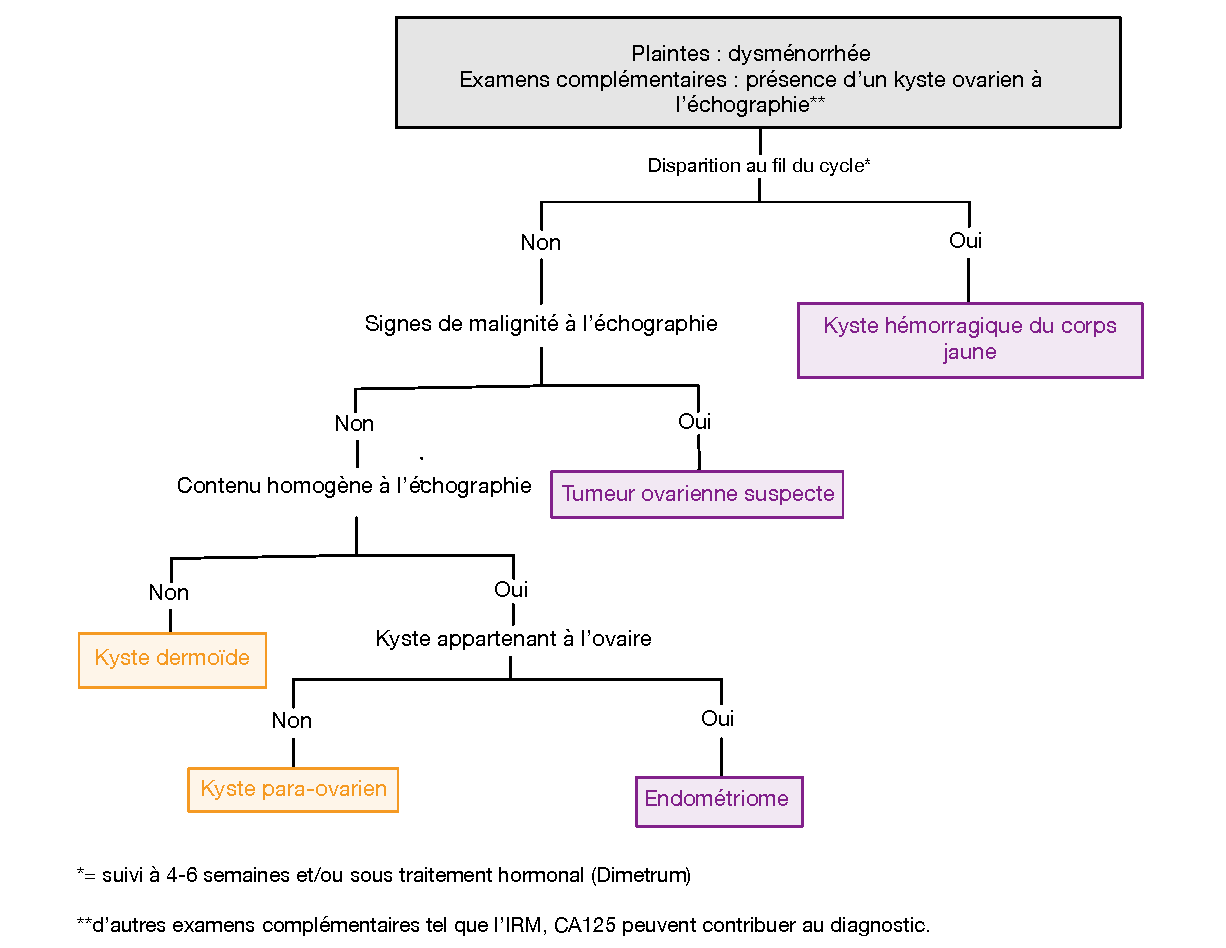
\includegraphics[width=14cm]{figures/01-cas-diagnostique/schema_DD.pdf}
    \end{tcolorbox}
    \caption{Arbre décisionnel des diagnostics différentiels d’un kyste ovarien chez une femme jeune en fonction de l’image échographique}
    \label{fig:ArbreDecisionMedical}
\end{figure}

\newpage

\subsection{Examen clinique} 
En gynécologie, l’examen clinique est souvent pauvre et il est nécessaire d’avoir une imagerie. Chez cette patiente, une palpation de l’abdomen a été réalisé. L’abdomen est souple, sans masse palpable. Toutefois, le toucher vaginal n’a pas été réalisé lors de la consultation car la patiente est vierge. Pourtant, un toucher vaginal pourrait donner des indications sur l’étendue de la pathologie. En effet, savoir qu’une mobilisation utérine est douloureuse ou la palpation d’autres masses éventuelles au niveau du ligament utéro-sacré, cul-de-sac de Douglas, \ldots{ } peut aider à orienter le diagnostic.

\subsection{Examens complémentaires}

\subsubsection{Biologie}
\begin{itemize}[label=\textbullet]
    \item \textbf{Justification :}\\
    une biologie a été réalisée dans le but d’évaluer le marqueur CA $125$, marqueur de l’irritation péritonéale. Son élévation est non spécifique mais présente lors d’endométriose profonde. La réserve ovarienne de la patiente est également estimé via l’AMH. Cette information aide à la prise de décision chirurgicale entre une kystectomie ou une annexectomie totale. L’hémoglobine et la coagulation sont aussi mesurées en cas de suspicion d’hémorragie intra-péritonéale et dans un contexte préopératoire proche.
    
    \item \textbf{Résultat :}%\\[0.3cm]
        \begin{table}[htbp]
\centering
\caption{Biologie - résultats}
\label{tab:examens_complementaires_resultat}
%\captionof{table}{Biologie - résultats}
\begin{tabular}{|p{0.2\textwidth}| p{0.2\textwidth}| p{0.2\textwidth}|}
    \toprule
    Nom & Quantité & Norme \\
    \midrule
    \hline
    AMH            & \qty{3.49}{\ug\per\L}           & \qtyrange{1.18}{9.2}{\ug\per\L} \\
    \hline
    CA 125         & \qty{82}{\kilo\enzymU\per\L}    & <~\qty{35}{\kilo\enzymU\per\L} \\
    \hline
    Hb             & \qty{13.2}{\g\per\dL}           & \qtyrange{11.5}{16.5}{\g\per\dL} \\
    \hline
    PT (quick)     & \qty{92}{\percent}              & >~\qty{70}{\percent}, T25--35 \\
    \hline
    INR            & 1                               & 1, T2.0--3.5 \\
    \hline
    aPTT           & \qty{29.8}{\second}             & \qtyrange{24.8}{34.4}{\second} \\
    \hline
    Fibrinogène    & \qty{262}{\mg\per\dL}           & \qtyrange{200}{400}{\mg\per\dL} \\
    \hline
\end{tabular}
\end{table}
        %\\[1cm]
        
    \item \textbf{Impact :}\\
    L’interprétation de l’élévation de CA $125$ est complexe vu son aspécificité. Certes, lors d’endométriose profonde, le marqueur augmente mais c’est également le cas lors d’un cancer ovarien ou même lors d’un kyste fonctionnel provoquant une irritation péritonéale. Selon les autres examens, cette donnée pourra appuyer le diagnostic sans avoir un impact décisif sur celui-ci.
    
\end{itemize}

\subsubsection{Imagerie}

\begin{itemize}[label=\textbullet]
    \item \textbf{Justification :}\\
    Afin de poser le diagnostic, une échographie sera réalisée $5$ semaines après la première imagerie. Cet intervalle permet d’apprécier l’évolution du kyste. Pendant l’intervalle libre entre les deux imageries, la patiente prendra une pilule progestative, Dimetrum\textregistered dont sa principale indication thérapeutique est l’endométriose. Le Dime\-trum\textregistered\ est une pilule en continu, il induira une aménorrhée chez la patiente et inhibera l’ovulation ce qui exclura le kyste fonctionnel s’il persiste. Le Dimetrum\textregistered\ induit un environnement hypo-œstrogénique et hyperprogestogénique, ce qui entraîne une atrophie de l'endomètre eutopique et ectopique, diminuant ainsi les dysménorrhées. Un traitement hormonal joue donc un rôle diagnostic mais également thérapeutique.
    
    \item \textbf{Résultat :}\\
    Il est important de notifier que la patiente a affirmé avoir eu ses menstruations lors des $5$ semaines séparant les deux imageries. Ceci indique que la patiente n’a pas été compliante sur la prise du Dimetrum\textregistered.\, A l’échographie, le kyste ovarien gauche persiste. Il s’agit d’un kyste de $63\,x\,53\,x\,59$ mm uniloculaire avec des parois fines continues et finement échogènes ainsi qu’un Doppler négatif. En résumé, l’imagerie obtenue ne répond à aucun critère de malignité (taille > $6$ mm, paroi épaisse, présence de septa, présence d’ascite, présence d’hétérogénéité au sein de la masse annexielle)
    
    \item \textbf{Impact :}\\
    La persistance du kyste exclut définitivement le kyste hémorragique du corps jaune. Les caractéristiques du kyste sont bégnines. L’image et le contexte clinique sont fortement compatibles avec l’endométriome.
\end{itemize}

\subsubsection*{Justification de l'evidence-based diagnosis}
\addcontentsline{toc}{subsubsection}{Justification de l'evidence-based diagnosis}
La plupart des examens complémentaires réalisés sont cliniquement justifiés dans le cadre du diagnostic d’un endométriome. Cette approche est soutenue par de nombreux éléments retrouvés dans la littérature médicale. J’ai pu trouver une étude clinique, \textcite{nieva2024impact}, qui questionnait sur l’impact de l’évolution des guidelines du diagnostic de l’endométriose. Historiquement, la laparoscopie était le gold standard pour diagnostiquer \todoH[TestStyle][green!30]{redondance et test de l'eapce commentaire à son maximum. Je t aime mon petit coeur de beurre. fjrea rgfre frf fr' frfa fraf frf 'hyh-' 'hgh fdnhdn hdngfd gd rehth erhg dngdb gehte h treht reh trehter h re hg erh ter ht hetr h  etgh getrh etyhtre hetrh htre htyh tek iut; u u, ut rzercz reb gtzrg gtrze rztre tgre regt tgt regtre tgrzeg treg trzg trgt rzg trzg trzg trzg tres grs gtr gtrze gtre zgtre zgt reg treg trz gtrz gt rzg trzg trz gtrz gt  grrg tre gtr eg treg tre gtr egt reg trzg trz gtre gt ergt reg t reg treg tre gt reg tre gt rz ze g rtv r trgt rgtregter tgre gtreg treg tregtreg gtrzg trz gtr g trzg trg tre tr eg  tzrgtr e tgre g trerteg tgr  rtg t rg trzg trz tg erg tre tgre  retgtr tr eg tre gtre t reg re trg e gt re gt re gt re}{l’endométriose}. Cette méthode présente pourtant des risques et les patientes y sont parfois réticentes. De plus, le lien de causalité entre l’étendue des lésions et la sévérité des symptômes reste incertain et complexe. D’autres inquiétudes apparaissent face à la laparoscopie qui pourrait retarder le diagnostic, voire sous-diagnostiquer les patientes. Donc, de nouvelles guidelines ont été établies par «European Society of Human Reproduction end Embryology» (ESHRE). Une approche multimodale a été adoptée, celle-ci prend en compte les symptômes des patientes ainsi que l’échographie transvaginale et l’IRM en complément de la laparoscopie pour diagnostiquer l’endométriose.  Les conclusions de cette étude clinique attestent que les recommandations, même les plus récentes, ont des limites. Elles ne permettent notamment pas de diagnostiquer l'ensemble des patientes en raison de l'hétérogénéité de la maladie et de ses symptômes. Il apparaît donc nécessaire d'élargir les critères et de replacer les symptômes au cœur de la démarche diagnostique. Cependant, l’évolution des guidelines a permis un diagnostic plus précoce par rapport à la laparoscopie seule mais cela n’est pas encore suffisant et de nombreux défis persistent.

Une autre méta-analyse, \textcite{kanti2024ultrasound}, a voulu comparer l’échographie transvaginale à l’IRM pour diagnostiquer l’endométriome. A nouveau, les différents essais cliniques qui confrontaient ces deux techniques étaient sujet à de nombreux biais. La comparaison de ces $2$ méthodes n’est donc pas évidente au niveau clinique vu le nombre d’études disponibles et leur qualité. Des critères peuvent, cependant, entrer en jeu tel que le coût, la disponibilité, \ldots{ } L’article tend à démontrer qu’il faut réaliser davantage d’études de comparaison mais que l’échographie et l’IRM sont deux imageries compétentes dans le diagnostic. Chacune des méthodes ayant leur avantages et inconvénients. Par exemple, l’échographie est plus accessible et moins onéreuse mais semble avoir un nombre de faux-positif plus élevé que l’IRM et donc moins spécifique. Dans notre cas, l’échographie était l’imagerie de choix vu son accessibilité et vu l’image détaillée et claire que nous avons obtenue. De plus, la laparoscopie thérapeutique permettra une seconde évaluation suffisante. L’IRM n’a donc pas sa place dans ce contexte.

Une étude multicentrique récente, \textcite{burghaus2024}\mbox{, }a évalué l’apport des biomarqueurs sanguins, notamment le CA $125$, dans le diagnostic de l’endométriose et de l’adénomyose. Les auteurs concluent qu’aucun biomarqueur seul ne permet actuellement de confirmer ou d’exclure avec certitude une endométriose. Toutefois, ils soulignent que le CA $125$ présente une bonne valeur diagnostique dans les formes sévères, en particulier en présence d’adhérences pelviennes ou d’un endométriome. En revanche, son utilité clinique diminue nettement dans les  autres formes. En cohérence avec ces limites, les recommandations du NICE et de l’ESHRE ne préconisent pas le dosage du CA $125$ comme outil diagnostique isolé, en raison de sa faible sensibilité et de sa variabilité interindividuelle. Dans notre cas, le dosage a été effectué, mais son interprétation reste délicate, et il n’apporte pas d’élément discriminant majeur dans la démarche diagnostique. Cet examen n’est pas inapproprié, mais il doit être interprété avec prudence et en complément d'autres éléments cliniques et radiologiques.

Pour aller plus loin dans la réflexion diagnostic, d’autres études comme \textcite{jiang2022diagnosis} questionnent l’utilité de l’intelligence artificielle dans le diagnostic de l’endométriose. Ceci est une preuve que de nouvelles pistes telles que l’intelligence artificielle doivent être explorées  car cette pathologie est encore trop souvent sous-diagnostiquée.

\subsection{Diagnostic}

\subsubsection{Diagnostic et sa présentation}
Le tableau clinique ainsi que les résultats obtenus lors des examens complémentaires sont grandement compatibles avec le diagnostic d’endométriome. L’endométriome est une forme particulière de l’endométriose. Cette maladie qui est la forme la plus fréquente et aussi appelée endométriome, est caractérisée par la présence de stroma et de glandes endométriales ectopiques notamment au niveau des ovaires. Ce kyste contient du sang couleur «chocolat» qui correspond à du vieux sang. L’endomètre ectopique est hormono-sensible et prolifère sous estrogènes pour se dégrader sous progestérone, tout comme l’utérus au cours du cycle. Le «vieux sang» correspond à la dégradation de l’endomètre qui ne peut être évacué et qui induirait des dysménorrhées.

\subsubsection{Ses répercussions}
Cette pathologie a un impact important sur le quotidien de la patiente. Les dysménorrhées ainsi que les autres symptômes empêchent la patiente d’assurer son quotidien. Son absentéisme professionnel a directement des conséquences négatives sur sa vie. Elle est sujet à la stigmatisation «des douleurs de règles». De plus, l’endométriome peut diminuer la fertilité voire rendre infertile la patiente.

\subsubsection{Traitement prescrit}
Deux alternatives de traitements ont été proposées à la patiente. D’une part un traitement de première ligne, un traitement hormonal, pour stabiliser la situation. Cependant, il s’agit d’un traitement symptomatique et il existe un risque d’expansion de la malade au niveau des trompes et des ovaires ce qui pourrait impacter davantage la fertilité. D’autre part, un traitement chirurgical par laparoscopie qui sera choisi par la patiente. Les indications de la chirurgie sont la dysménorrhée et le désir de grossesse. Vu la réserve ovarienne et l’âge de la patiente, une kystectomie est préférable à une annexectomie. La taille du kyste étant supérieure à 5mm, une kystectomie en deux temps peut être nécessaire avec une prise d’antagoniste GnRH entre les deux interventions dans le but d’atrophier les lésions endométriales. La laparoscopie permet également d’observer la cavité abdominale et de s’assurer que l’endométriose n’a pas envahi celle-ci.
\section{Communication au patient}

\subsection{Endométriome}
Endométriome est une maladie complexe. Il s’agit d’un type d’endométriose. Cela signifie qu’au niveau des ovaires, nous retrouvons un kyste rempli de liquide. Ce kyste contient entre autres de l’endomètre qui est la muqueuse de l’utérus, ce qui est une localisation anormale. La douleur qui revient chaque mois s’explique parce que le kyste réagit comme l’utérus au cours du cycle menstruel, c’est-à-dire qu’il se construit, prolifère au cours de la première phase du cycle et s’auto-détruit à la fin du cycle ce qui correspond aux règles au niveau de l’utérus. Cependant, le tissu utérin étant au niveau du kyste ne peut pas s’évacuer, le sang va donc s’accumuler et provoquer des douleurs intenses. L’endométriome est une lésion bégnine, mais pouvant entraîner des complications fonctionnelles importantes, notamment sur la fertilité.

\subsection{Symptômes}

%\begin{singlespace}
Les symptômes typiques sont:

\begin{itemize}[compact, label=\textbullet]
    \item Douleurs intenses lors des menstruations qui impact le quotidien de la patiente;
    \item Douleurs pelviennes;
    \item Douleurs lors des rapports sexuels;
    \item Douleurs lors de l’évacuation des selles ou parfois des urines;
    \item Troubles de la fertilité;
\end{itemize}
%\end{singlespace}

La présence de ces symptômes ne signifie pas systématiquement la présence d’endométriose mais justifie une évaluation avec un gynécologue expérimenté. Il convient de noter que tous ces symptômes ne sont pas toujours présents et qu’ils fluctuent énormément selon chaque patiente. Dans ce cas, la patiente ressent de vives douleurs lors de ses menstruations depuis de longtemps et qui se sont accentuées ces 4 derniers mois.

\subsection{Diagnostic}
Le diagnostic de cette patiente a pu être posé en observant l’évolution du kyste appréciable grâce aux différentes imageries réalisées et à la prise de la pilule Dimetrum\textregistered.\, De plus, le marqueur CA 125, étant élevé, confirme notre diagnostic.

\subsection{Traitement}
Le traitement consiste en une intervention au cours de laquelle le chirurgien enlève toutes les lésions endométriales visibles. L’opération ne laisse que trois petits trous au niveau abdominal utiles pour le passage des instruments. Ensuite, le ventre de la patiente va être gonflé d’air afin d’avoir une meilleure vision. Une fois le kyste visible, le chirurgien pourra commencer sa résection. Si d’autres lésions sont visibles, le chirurgien en profitera pour faire un traitement global. Si l’endométriome est trop conséquent et que les ovaires risquent d’être trop endommagés, la chirurgie se fera en deux temps. Entre ces deux interventions, la patiente devra prendre un traitement hormonal afin de réduire la taille des lésions restantes ce qui facilitera la seconde chirurgie.

\subsection{Suivi}
Le suivi commence par une consultation post-opératoire afin de vérifier les plaintes éventuelles de la patiente ainsi que l’évolution de la cicatrisation au niveau ovarien. Une imagerie de contrôle sera réalisée entre 3 à 6 mois ainsi qu’une réévaluation de la réserve ovarienne à posteriori. D’autres suivis peuvent être organisés selon la volonté de la patiente tel qu’un suivi de fertilité, un suivi hormonal s'il y a un désir d’aménorrhée.
\section{Approche réflexive}

\subsection{Si vous deviez ne retenir qu’une seule notion de ce travail, quelle serait-elle ?}
Les dysménorrhées doivent être explorées par le médecin. Trop souvent, les patientes traversent un désert diagnostique, ne se sentent pas soutenues ni écoutées. La première mission d’un médecin est de soigner un patient et non une pathologie. Apporter un maximum de confort aux patients est l'objectif.

\subsection{Que pensez-vous avoir bien réussi dans ce travail ?}
Je pense que ce cas clinique n’est pas un cas diagnostique idéal vu l’examen clinique pauvre et les diagnostics différentiels peu nombreux. D’autres cas auraient été plus évidents. Toutefois, cela m’a poussée à me renseigner davantage sur les différentes kystes ovariens possibles. Je pense, par contre, avoir gardé une structure claire tout au long du travail facilitant ainsi la compréhension. La recherche réalisée sur PubMed m’a grandement aidé pour appuyer la démarche diagnostique. Lire ces études m'a permis de mieux comprendre le contexte médical et les enjeux des différents examens cliniques possibles, leurs avantages et inconvénients. Être à jour au niveau de la littérature médicale est un avantage certain car elle permet un choix éclairé et optimal pour la patiente.

\subsection{Que pensez-vous devoir améliorer ?}
Je pense pouvoir améliorer la formulation de mes phrases, afin de les rendre plus médicalisées et précises. J’ai tenté au maximun d'utiliser le jargon médical, mais je suis convaincue qu’avec l’expérience, je parviendrai à m’exprimer de manière plus concise et rigoureuse. Lors de l’anamnèse, je ne suis pas toujours certaine de la pertinence des informations récoltées.

Le contexte socio-économique et les antécédents médicaux, notamment lorsqu’ils concernent un séjour à l’étranger, ont été peu développés dans ce travail en raison de données manquantes. La barrière de la langue représente également un obstacle à une communication optimale avec la patiente. Il aurait été pertinent d’obtenir davantage d’informations objectives sur les douleurs pelviennes rapportées depuis 7 ans.

\subsection{Quelle(s) question(s) souhaiteriez-vous approfondir dans un prochain travail ?}
L’aspect thérapeutique de la démarche clinique, particulièrement dans le cadre d’une pathologie chronique, est un point que je souhaiterais approfondir. Aujourd’hui encore, les liens entre lésions et symptomatologie ne sont pas toujours scientifiquement établis, ce qui explique les multiples options thérapeutiques proposées aux patientes.

J’aurais apprécié pouvoir suivre l’évolution de la patiente et comprendre son choix de s’orienter vers une solution chirurgicale. Ouvrir la discussion sur d’éventuelles alternatives aurait été enrichissant, tant pour elle que pour moi en tant que future médecin. Explorer ces dimensions aurait apporté une valeur ajoutée à ce travail.

\geometrieLarge
\begin{figure}
  \centering
  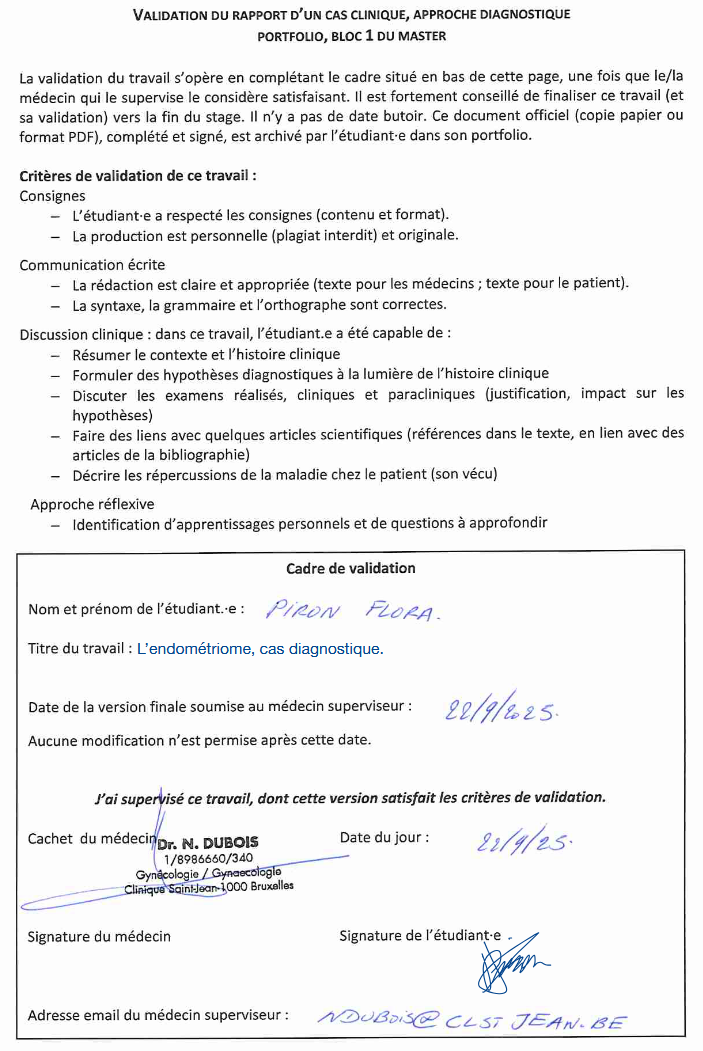
\includegraphics[width=0.9\textwidth]{figures/01-cas-diagnostique/fiche_validation_DrDuboisV2.png}
  \caption{fiche validation}
  \label{fig:fiche_validation_DrDubois}
\end{figure}
\geometrieWord


\includepdf[pages=1, pagecommand={\thispagestyle{empty}}]{figures/covers/FP_Page_de_garde_page_03.pdf}


\chapter{Activité extérieure}

Spectacle de danse : Yé ! (L’Eau), par Circus Baobab, 23 novembre 2024 à la Maison de la culture d’Arlon. 
Dr. P. Jacquemart

\section{Résumé et justification de l'activité}

\todoH[FloraStyle][red!30]{\ les corps du spectacle  sont différents par rapport à l’europe (choix pe des gens plus filiformes dans les compagnies europiénnes) pe ajouter une ligne sur ce thème}{}

L’activité culturelle que je souhaite détailler est un spectacle de \todoH[FloraStyle][red!30]{\ est-ce que c'est la bonne façon de citer ou i faut mettre en textcite ?? }{danse, Yé ! (L’Eau)} \parencite{circusbaobab_site}. La danse est un moyen de communication unique soumis à l’interprétation de chacun. Cet art requiert une certaine sensibilité et imagination afin d’en comprendre toute son histoire. Apprendre à voir au-delà, comprendre un message au travers des lignes du corps au lieu de celles des livres. La danse est un moyen d’ouvrir l’esprit afin de mieux comprendre l’autre. Tout le monde n’a pas le même langage et pourtant en suivant la gestuelle de la danse, une union se fait entre les spectateurs et les danseurs.  Ayant moi-même pratiqué la danse, je ne pouvais qu’admirer tous ces corps se mouvant à l'unisson. Poids plume, les danseurs étaient impressionnants et au-delà de la prouesse physique, ils ont, selon moi, su transmettre un message fort.
 
Yé ! représente avec force la question de nos ressources actuelles, et leur absence cruelle dans certaines régions du monde. Les danseurs se battent pour atteindre cette eau inaccessible. Ils représentent les Hommes qui se réinventent, construisent mais se déconstruisent également entre eux au nom de la santé, de la vie. Ces voltigeurs créent de véritables pyramides humaines aussi fortes que fragiles grâce à un équilibre étroit. A travers ce spectacle, les danseurs tentent de nous transporter et de nous transmettre l’espoir d’un avenir meilleur. Si, ensemble, nous agissons malgré une situation actuelle plus qu’alarmante. La thématique environnementale était rythmée par la friction des bouteilles en plastique, symboles percutants de la crise climatique actuelle et le fardeau de nos déchets. En effet, le décor était plus que minimaliste, un tapis de bouteilles était l’unique accessoire des danseurs. Loin d’un ballet classique, le contemporain permet une plus grande liberté d’expression et de mouvements. Une empreinte circassienne a également imprégné cette performance.
 
L’un des points de vue inspirants de ce spectacle est la place qu’il accorde à ses danseurs en tant qu’individus et artistes. En effet, le Circus Baobab est une troupe de cirque itinérante. Il a vu le jour en Guinée grâce à Laurent Chevallier, un célèbre réalisateur de cinéma. La compagnie permet à de nombreux danseurs d’avoir un métier stable et de sortir de la précarité. Alors qu'au départ, leur tournée ne s’étendait qu’aux villages environnants, de nos jours, ils traversent toute la France et ses pays limitrophes pour s’exprimer et faire voyager les spectateurs à travers la danse. Ils utilisent les réseaux sociaux pour faire connaître leur cause. Ils n’hésitent pas à montrer leur engagement auprès des plus jeunes car ils recrutent régulièrement. Ils publient également les heures d’entraînement passées afin de nous faire vivre une expérience hors norme ainsi que leur succès et toutes les différentes populations qu’ils ont réussi à toucher avec leurs messages. En outre, ces représentations révèlent des silhouettes rarement observées au sein des compagnies européennes, elles constituent ainsi une invitation à la tolérance et à l'acceptation de la pluralité des corps.

Lorsque le rideau tombe, une réflexion naît. Une fois de plus c’est un rappel de la chance que nous avons dans notre pays, d'avoir des ressources et un système de santé aussi développés tout en ajoutant une touche de culpabilité car si d’autres régions sont moins chanceuses, des actions peuvent être faites chez nous pour changer les choses. Avoir un rappel aussi délicat et artistique permet d’écouter le message sans se sentir impuissant. De plus, sachant l’histoire de la compagnie, se dire qu’en regardant simplement un spectacle nous rendons possibles à ces danseurs de continuer leur route et de soutenir leurs actions. Ce spectacle ne demande qu’à être regardé, écouté et à ouvrir la porte à la réflexion.

En dehors du cadre académique, je suis convaincue qu’il est primordial d’être ouvert à d’autres façons d’apprendre et de voir le monde. Spécialement dans notre médecine actuelle qui fait face à bien plus de \todoH[FloraStyle][red!30]{\ défis ? lesquels frustrations de pas les détailler, changer la formulation pour fermer les propositions  }{défis} que les soins du patient. Parmi ces défis, je peux notamment citer l'élaboration particulière de la relation patient-médecin ou encore la conscience de la santé planétaire et les aspects économiques des soins.
\section{Impact sur ma pratique future}

Bien que la connaissance factuelle et la rigueur soient des fondements essentiels de la pratique médicale, compte tenu des enjeux vitaux, il serait réducteur de s'arrêter là. Ne risquons-nous pas de perdre l'essence de la relation humaine si nous échouons à décoder ce qui se transmet au-delà du verbal ? Le langage non-verbal est, en effet, aussi un vecteur fondamental de la communication médecin-patient. À cet égard, la célèbre théorie d'Albert Mehrabian \parencite{demetersante2022}, qui attribue une part prépondérante au non-verbal ($55$\% pour le langage corporel) dans la communication des attitudes et des émotions, confirme l'impératif de développer cette compétence. Apprendre à interpréter les signaux corporels du patient devient alors une composante nécéssaire à notre formation. Ce besoin est amplifié face aux patients dont l'expression est limitée par des facteurs tels que l'âge, la langue, la culture ou la pathologie. La danse, en tant qu'expression corporelle par excellence, représente ainsi une éducation précieuse à l'observation fine de l'autre.

\todoH[FloraStyle][red!30]{\ passage trop stigmatisant. MG médecine environnementale !!! apporter des nuances }{\mbox{Au-delà de l'émotion artistique}}, cette expérience invite aussi à explorer le concept du One Health défini par une approche systémique reconnaissant que la santé humaine, la santé animale et l'équilibre des écosystèmes sont fondamentalement interdépendants. L’antibiorésistance illustre parfaitement la nécessité de cette approche. Face à cette menace, les mesures traditionnelles de la médecine humaine (contrôle des prescriptions, recherche, hygiène hospitalière) restent insuffisantes. Le One Health impose une vision systémique et multidisciplinaire. Concrètement, cela implique d'optimiser les prescriptions médicales et vétérinaires, mais aussi d'améliorer le traitement des \todoH[FloraStyle][red!30]{\ perturbateurs endocriniens dans les eaux usées pas que AB --> il y a plein d'exemples possibles mais questions de nombre de mots, je ne vais pas en parler}{eaux usées} pour y réduire la concentration d’antibiotiques et de bactéries résistantes. L'éducation et la prévention auprès de tous ces professionnels (soignants, vétérinaires, agriculteurs) sont également primordiales. Heureusement, des transitions s'opèrent déjà dans l'enseignement professionnel : en Belgique, l'utilisation des huiles essentielles \parencite{siep_formation_524} en agronomie est enseignée comme alternative aux antibiotiques en élevage, avec des plans d'actions aux résultats encourageants selon \textcite{celagri_antibioresistance}.\\
Je suis convaincue que l’intégration du One Health représente l’avenir d'une médecine engagée et préventive, vers laquelle notre formation tend de plus en plus. À notre échelle, des gestes cliniques modestes (une anamnèse approfondie, un examen rigoureux et une prescription réfléchie avant tout examen complémentaire) contribuent déjà à une pratique plus durable et à la transformation globale de notre manière de soigner.


Certes, cette vision peut sembler idéaliste, mais elle est porteuse d’espoir. Même si cette transition vers une médecine plus responsable ne se fera pas en un jour, elle se fera. Ce "micro-rappel" précieux nous recentre sur l’essentiel et nous ouvre à une réflexion plus large sur notre mission de soignant.
\section{Conclusion}

Vous présenter un spectacle de danse rappelle que soigner, c’est avant tout écouter sans parole et accueillir sans jugement. J’ai été profondément touchée par l'engagement de cette troupe modeste, qui porte un message fort tout en transformant concrètement l'avenir de ses jeunes danseurs. En ajoutant la thématique du OneHealth qui est un sujet incontournable dans notre médecine moderne et l’aborder à travers la danse est une idée qui me correspond. Cette perspective globale du soin, à la fois intime et planétaire, est une conviction que je souhaite garder tout au long de ma formation et de ma pratique future.

\geometrieLarge
\begin{figure}
  \centering
  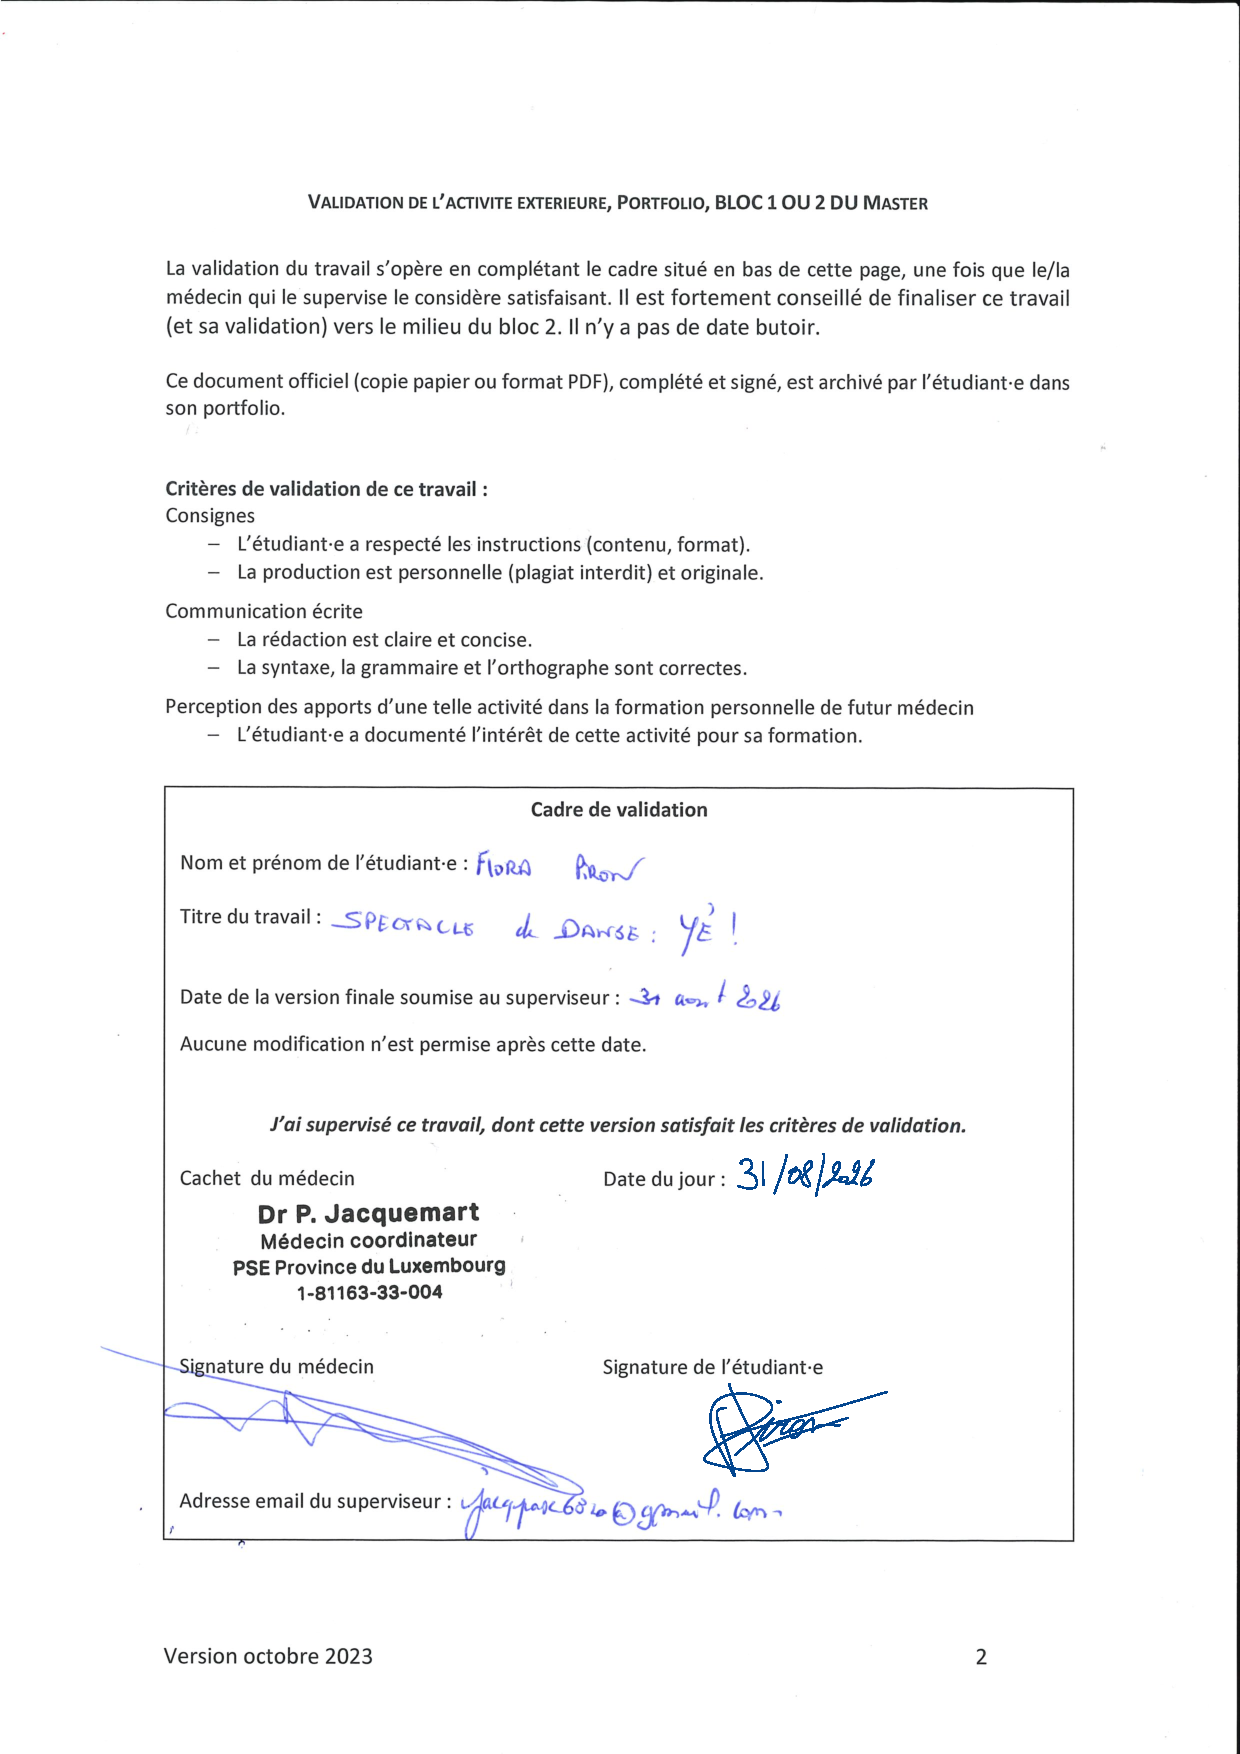
\includegraphics[width=0.9\textwidth]{figures/02-activite-exterieure/FicheValidation_ActExt.pdf}
  \caption{fiche validation}
  \label{fig:fiche_validation_DrJacquemart}
\end{figure}
\geometrieWord


\includepdf[pages=1, pagecommand={\thispagestyle{empty}}]{figures/covers/FP_Page_de_garde_page_04.pdf}


\chapter{Cas thérapeutique}

\section{Résumé du cas clinique}

\subsection{Motif}
La patiente se présente aux urgences, le 30 décembre 2025, accompagnée de la police pour une demande d’internement à la suite d'une tentative de suicide.

\subsection{Contexte social}
La patiente a 60 ans, elle a un fils de 27 ans. Elle s’est séparée du père lorsque celle-ci était encore enceinte. Depuis madame vit seule avec son fils.

Au niveau professionnel, elle est pensionnée depuis le 1 janvier 2026. Elle a fait carrière en tant que secrétaire de direction.

La patiente rapporte avoir été victime de violence dans son enfance. 
Ensuite, son ancien compagnon était violent avec elle. De plus, l’enfant est issu d’un viol de celui-ci. Elle a toutefois, décidé de se séparer de cet homme tout en gardant l’enfant et en l’élevant en tant que mère célibataire. Actuellement elle subit des violences physiques et verbales de la part de son fils rendant la situation intenable au domicile. Celui-ci a été diagnostiqué dès son plus jeune âge de trouble de l’attention et d’hyperactivité ainsi que du trouble du spectre autistique. En effet, il présente un comportement violant à la moindre contrariété. Celui-ci a un suivi psychiatrique mais n’a pas de situation professionnelle ni logement.

\subsection{Antécédents psychiatriques}
\begin{itemize}[label=\textbullet]
    \item \underLine{Depuis l’âge de 18 ans} : dépression récurrente.
    \item  \underLine{De 2015 à 2021 } : suivi psychiatrique mais aucun suivi ambulatoire depuis.
    \item \underLine{ 2021} : dépendance aux benzodiazépines.
    \item \underLine{ 2021 et juillet 2025} : 2 hospitalisations pour dépression.
\end{itemize}

\subsection{Antécédents somatiques}
\begin{itemize}[label=\textbullet]
    \item Actuellement en rémission d’un mélanome.
    \item Thyroïdite d’Hashimoto  
    \item Fibromyalgie
    \item Vessie hypertonique
    \item Diarrhées chroniques idiopathiques
\end{itemize}

\subsection{Allergies}
\begin{itemize}[label=\textbullet]
    \item Moxifloxacine 
\end{itemize}
 
\subsection{Antécédents familiaux}
\begin{itemize}[label=\textbullet]
    \item Son père affecté d’un cancer prostatique au stade métastatique. 
\end{itemize}

\subsection{Anamnèse}  
Suite à une tentative d’étranglement de la part de son fils, la patiente aurait fait une tentative de suicide. La patiente dit avoir pris 5--6 comprimés de lormétazépam \qty{2}{\mg}, 6--7 comprimés de lorazépam \qty{1}{\mg}, 2 comprimés d'alprazolam retard dont la dose est inconnue. Elle aurait été retrouvée inconsciente à l’arrivée de la Police qui avait été prévenue par les voisins. Elle souhaite inscrire son fils auprès d’associations qui pourraient l’aider à trouver un logement et un travail mais les délais d’attente sont longs. La patiente ne voit pas de solutions possibles à court terme. Malgré la thymie triste et les ruminations suicidaires qui persistent, la patiente se projette dans l’avenir et a des projets. 

\subsection{Examen clinique}
La patiente est anxieuse avec une thymie triste et labile.
Elle est cohérente. Une hypoprosexie est observée. 
Son discours est volubile et circonlocutoire pouvant témoigner d’une grande charge anxieuse associé à des difficultés d’attention et une accélération psychique. 
La patient présente des insomnies de maintien. 
Sur le plan psycho-affectif, on note une intense ambivalence vis-à-vis du fils. 
La patiente oscille entre un désir de protection maternelle, teinté de culpabilité, et un besoin de mise à distance vitale face aux hétéro-agressions subies. Cette dynamique relationnelle complexe alimente un sentiment d'impasse existentielle, majorant le risque suicidaire. 
Une hyper-émotivité est observée chez la patiente ce qui se perçoit comme une personne qui s’implique beaucoup avec les personnes qui sont bienveillantes avec elle. 

\subsection{Examens complémentaires}
\begin{itemize}[label=\textbullet]
    \item Biologie : sans particularité mis à part une hypercholestérolémie à \qty{243}{\mg\per\dL}. (Ionogramme et fonction rénale (>~\qty{60}{\mL\per\minute}) sont corrects).
    \item ECG : rythme sinusal, FC \qty{80}{\bpm}
\end{itemize}
Voir détails des examens complémentaires en \cref{annexe:examens_complementaires} en \cpageref{annexe:examens_complementaires}.

\subsection{Diagnostic retenu}
 
Épisode dépressif majeur avec caractéristiques mixtes\footnote{\url{https://www.infodrog.ch/files/content/refbases/DSM-5_Manuel-diagnostique-et-statistique-des-troubles-mentaux.pdf\#page=286} \parencite{dsm5_online}}  dans un contexte familial relationnel difficile.

\subsection{Traitements réalisés et prise en charge} 
\begin{itemize}[label=\textbullet]
    \item Paroxétine (Seroxat)  \qty{20}{\mg} 1 cp/j
    \item Zopiclone (Imovane) \qty{7.5}{\mg} 1 cp/j
    \item Olanzapine (Zyprexa) \qty{5}{\mg} 1 cp/j 
    \item Lorazépam (Temesta) \qty{2.5}{\mg} 1 cp/j
    \item Lévothyroxine sodique (T4, \qty{100}{\ug}) et liothyronine sodique (T3, \qty{20}{\ug}) (Euthyral) \qty{75}{\mg} 1 cp/j 
    \item Lopéramide (Imodium) \qty{2}{\mg} 2 cp/j
    \item Fésotérodine (Toviaz) \qty{4}{\mg} 1 cp/j 
\end{itemize}
 
Ce traitement pharmacologique est associé à une psychothérapie et l’hospitalisation sera suivi d’une cure psychothérapeutique stationnaire. 
Une assistante sociale s’intéresse également au cas afin de tenter d’apporter des solutions dans la sphère sociale de la patiente. 
 
Lors de l’hospitalisation, un changement au niveau du traitement a eu lieu. Le valproate de sodium \qty{500}{\mg} a été remplacé par l’olanzapine \qty{5}{\mg} principalement à cause d’une chute de cheveux marquée lors de l’augmentation de la posologie du valproate. De l’olanzapine est mis à la place avec effet positif thymorégulateur et nette atténuation des fluctuations émotionnelles au cours d’une même journée. 
 
L’abandon de la quétiapine \qty{20}{\mg} a également eu lieu car elle a présenté des éruptions cutanées. 

\subsection{Évolution de l’hospitalisation }
Amélioration thymique et amélioration de son sommeil. 
La patiente a des idées noires passagères toutefois dans l’évolution de son hospitalisation, celle-ci demande de l’aide auprès des soignants. 
La patiente apprend a posé ses limites auprès de son entourage. 

\subsection{Ressenti de la patiente}
La patiente semble être demandeuse de traitement et a une volonté d’aller mieux. La patiente voit son hospitalisation comme un moyen se protéger de son fils et comme une ressource sociale pour l’aider dans les démarches administratives et trouver des solutions.
 
Concernant son traitement psychiatrique, la patiente associe cela à un même besoin qu’un traitement somatique. Elle a toujours considéré sa santé mentale au même titre que sa santé physique. Il est donc normal pour elle de prendre un traitement quotidiennement. 
La patiente se décrit comme une personne «hypersensible» pharmacologiquement parlant, en d’autres termes, avec le temps, elle a eu l’occasion de tester de nombreuses molécules différentes et selon elle, elle ressentirait les effets secondaires plus fréquemment que la population générale et avec des doses plus faibles. Au cours de sa prise en charge avec son psychiatre extérieur, elle dit n’avoir jamais trouvé l’équilibre entre bénéfices et effets secondaires, y compris avec le valproate. Depuis l’instauration de l’olanzapine, elle se sent mieux. 
\section{Démarche de médecine factuelle}

\subsection{Informations scientifiques}
  
\subsubsection{Méthode}

PICO :
\begin{itemize}[compact, label=\textbullet]
    \item Population : Patient souffrant d’un épisode dépressif résistant avec caractéristiques mixtes. 
    \item Intervention : l’ajout d’antipsychotiques au traitement antidépresseur. 
    \item Comparateur : placebo. 
    \item Outcome : obtenir une rémission des symptômes et prévenir les effets secondaires. 
\end{itemize}

Banque de données consultée : Pub Med.\\ 
Termes MeSH utilisés : «Major Depressive Disorder », «Mania» et «Antipsychotic Agents».\\
Critère pour la sélection d’article : publication dans les 5 ans, «Free full text», «Randomized controlled trial», «Meta-analyse» et «Systematic review».\\
Date de consultation et nombre d’articles : le 07 février 2026, 2 articles répondaient à ces critères. 

\subsubsection{Résultats}  

L'article choisi est le suivant, \textcite{gao2025efficacy}.
 
Les auteurs constatent une amélioration des symptômes dépressifs et maniaques avec les antipsychotiques chez les patients souffrant de MDE-MFS -- major depressive episodes with mixed features specifier. Ce traitement aurait un profil des effets secondaires bénéfiques sans risque augmenté d’effets secondaires sévères. Les stabilisateurs de l’humeur et certains antidépresseurs -- trazodone -- montreraient également une efficacité chez ces mêmes patients. Toutefois, la preuve de leur efficacité et leur sécurité étaient limitées et controversées dû au nombre restreint d’études disponibles.

\begin{figure}[H]
    \centering
    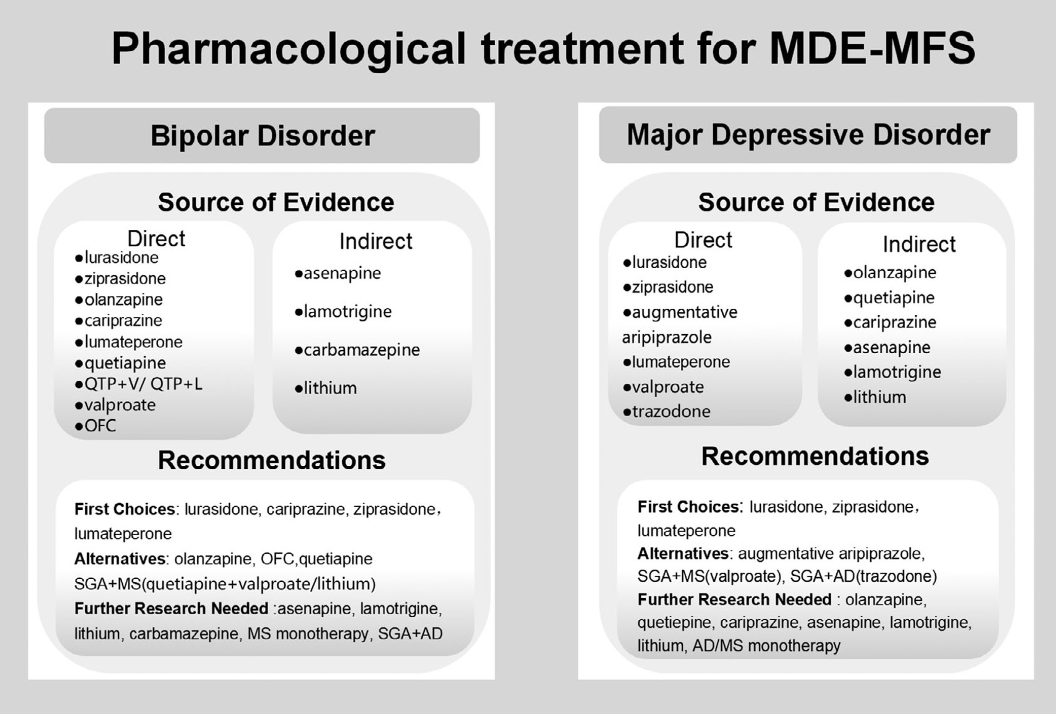
\includegraphics[width=\textwidth]{figures/03-cas-therapeutique/resultat_etude_casM2.png}
    \caption{traitement pharmacologique pour MDE-MFS}
    \label{fig:resultat_etude_casM2}
\end{figure}

\subsubsection{Discussion}





\begin{itemize}[label=\textbullet]
    \item \textbf{Analyse critique de la méthodologie}\\
    La méthodologie de cette méta-analyse, notamment pour évaluer puis stratifier les différents articles selon leur biais, semble complète et rigoureuse tout à fait en accord avec l’EBM. Pour chaque nature d’article, différents outils adaptés ont été employés \todoH[FloraStyle][red!30]{Cochrane tool (Higgins et al., 2011) : C'est le standard mondial ("gold standard") pour évaluer les biais dans les essais contrôlés randomisés (RCT). Il analyse précisément la randomisation et l'insu.
    Newcastle-Ottawa Scale (NOS) : C'est l'outil de référence pour les études observationnelles et les analyses post-hoc.
    ROBINS (Risk of Bias In Non-randomized Studies) : C'est l'outil le plus robuste recommandé par la collaboration Cochrane pour les études d'intervention non randomisées.
    Outils JBI (Joanna Briggs Institute) : Ils sont reconnus internationalement pour l'évaluation rigoureuse des séries de cas et des rapports de cas.}{(Cochrane pour les RCTs, NOS pour les études observationnelles, ROBINS pour les études ouvertes).}
    
    Concernant le biais de publication, il a été mesuré selon plusieurs outils, à nouveau pour argumenter et valider au mieux les résultats. Le funnel plot est cependant difficilement interprétable vu le nombre d’études sélectionnées inférieur à 10 mais le test d’Edgar avec $p \ge \num{0.05}$ confirme l’absence de biais de publication significatif.
    
    L’analyse de la sensibilité via la méthode «leave-one-out» a démontré qu’une étude en particulier, l'étude de Singh et al. (2020) sur les adolescents, déstabilisait les résultat concernant les symptômes maniaques et donc montre un $I^2$ élevé. Afin de résoudre cette forte hétérogénéité, cette étude a été exclue. 
    
    Les méthodes utilisées pour interpréter les résultats de cette méta-analyse semblent répondre à l’EBM. Toutefois, le talon d’Achille de cette étude est le nombre d’études disponibles et leur qualité intrinsèque, en effet la majorité des articles étaient des analyses post-hoc, c’est-à-dire, des analyses qui n’avaient pas pour objet la thématique de cette méta-analyse mais dont les données ont été recueillies. Les auteurs qualifient donc cette méta-analyse de préliminaire, nécessitant par la suite des RCT prospectifs. De plus, les variations de définition de dépression avec caractéristiques mixtes sont retrouvées dans la littérature médicale ce qui complique la réalisation de la méta-analyse et peut-être biaise la sélection des patients. 
    
    \item \textbf{L'interprétation des principaux résultats}\\
    Concernant les antipsychotiques, le taux de réponse clinique est meilleur par rapport au placebo  (RR = \num{1.46} [\qty{95}{\percent} CI: \num{1.31}, \num{1.61}], $p < \num{0.001}$; NNT = 7 [\qty{95}{\percent} CI: 5, 9]).  Les autres outcomes primaires tels que l’évolution du \todoH[FloraStyle][red!30]{\url{https://www.ciusss-capitalenationale.gouv.qc.ca/sites/d8/files/docs/ProfSante/Infirmier/evaluation-manie-young.pdf}}{score YMRS}, l’échelle d’évaluation de la manie de Young, montrent une nette réduction comparée au placebo (SMD = \num{0.35} [\qty{95}{\percent} CI: \num{0.53}, \num{0.17}], $p < \num{0.001}$). 
    
    Quant à l’outcome primaire de sécurité, TEM rate qui signifie le virage maniaque, n’est pas significativement différent du groupe contrôle (RR = \num{0.91} [\qty{95}{\percent} CI: \num{0.53}, \num{1.55}], $p = \num{0.65}$). Par contre, les antipsychotiques ont été associés à une recrudescence du risque d’effets secondairess classique par rapport au placebo (RR = \num{2.33} [\qty{95}{\percent} CI: \num{1.63}, \num{3.34}], $p < \num{0.001}$; NNH = 17 [\qty{95}{\percent} CI: 11, 25]) particulièrement pour les symptômes extrapyramidaux et le trouble de la vigilance et du sommeil.
    
    Les auteurs ont également analysé l’efficacité et la sécurité de différents types d’antipsychotiques chez les patients souffrant de d’épisodes dépressifs majeurs avec caractéristiques mixtes dans un contexte de dépression majeure. Cependant, le nombre restreint d'études disponibles pour ce profil clinique spécifique a limité les conclusions à une analyse descriptive, empêchant la réalisation d'une synthèse quantitative formelle. Malgré cette limite, les données révèlent une efficacité supérieure des antipsychotiques sur le placebo pour stabiliser les deux pôles de la pathologie. La lurasidone a notamment montré un taux de réponse supérieur au placebo (\qty{64.8}{\percent} versus \qty{30.0}{\percent}, $p < \num{0.001}$), avec une amélioration des symptômes maniaques confirmée à long terme.  Sur le plan de la sécurité, aucune augmentation significative du risque de virage maniaque (taux de TEM) ou de symptômes extrapyramidaux (EPS) n'a été observée par rapport au placebo, les effets indésirables courants comme la somnolence ou les nausées restant généralement modérés et tolérables.
    
    Toujours en reprenant cette population précise, une étude a montré une amélioration significative des symptômes dépressifs grâce aux stabilisateurs de l’humeur (valproate) à dose moyenne chez 18/22 patients. Lors du suivi, certains ont rapporté des effets secondaires et un tiers de ces personnes ont arrêté le traitement pour cette raison. Deux études rétrospectives indiquent enfin que la trazodone pourrait réduire efficacement l’agitation et les symptômes mixtes avec un profil de sécurité rassurant, bien que l’absence de groupe contrôle impose de considérer ces résultats comme préliminaires.
\end{itemize}
 
\subsubsection{Conclusion} 
 
Cet article confirme les guidelines et appuie la sécurité et l’efficacité des antipsychotiques, régulateur de l’humeur et de certains antidépresseurs dans ce contexte de MDD avec MDE-MFS. Toutefois, il faut garder à l’esprit les limites de cette méta-analyse notamment le nombre limité d’études disponibles et que les auteurs ont décidé d’inclure des analyses post-hoc. 
 
\subsection{Contextualisation}
La patiente, au cours de sa prise en charge, a souffert de nombreux effets secondaires. Certains s’associent à des pathologies déjà présentent, notamment les troubles de transites qui s’additionnent aux diarrhées chroniques idiopathiques. 

En pratique, vu les traitements antérieurs et leur tolérance chez la patiente, plusieurs molécules étaient éliminées dont la quétiapine, le valproate. Un régulateur de l’humeur était à envisager compte tenu des caractéristiques mixtes de sa dépression. L'olanzapine semblait donc une molécule de choix pour associé à la paroxetine vu son efficacité prouvée sur ce type de diagnostic. Cependant, l'hypercholestérolémie objectivée par le bilan biologique constitue un paramètre de vigilance majeur, car l'olanzapine est étroitement associée à un risque accru de dyslipidémie et de syndrome métabolique.

Si l’on suit les recommandations de la méta-analyse la lurasidone pourrait être également une alternative vu son profil d’efficacité et de tolérance dans la population MDD avec MDE-MFS. La trazodone pourrait également apporter des effets positifs chez la patiente, tout en s’assurant de la bonne tolérance de la patiente.

Il est important de noter que la patiente est compliante et vu son éducation thérapeutique et ses croyances, avoir un traitement comprenant plusieurs comprimés quotidiens ne représente pas un obstacle à la prise en charge.

La prise en charge de la patiente doit prendre en considération la sphère sociale. En particulier, le déclencheur principal de cette hospitalisation a été son fils. Par conséquence, la situation ne sera pas résolue tant que le fils habitera avec la patiente. C’est pourquoi une cure psychothérapeutique stationnaire a, en partie, été mise en place afin de solutionner temporairement le problème social et évidemment pour traiter la patiente au niveau psychologique. Le traitement médicamenteux a aussi son rôle à jouer pour stabiliser la patiente à court terme lorsque le travail psychologique et social se résout à long terme. 

\subsection{Intégration}
La littérature médicale permet de guider le praticien. Bien sûr les guidelines ont leur place dans la prise de décision du médecin. Cependant, la patiente doit être au centre des soins et elle n’est pas égale à la population générale. Il faut donc adapter sa prise en charge à la personne qui est souffre de la pathologie en question et l’adapter à son contexte social et familial. Dans ce cas, la patiente a besoin de prise en charge psychologique et sociale qui ne peuvent pas se résoudre rapidement. La décision d’un traitement médicamenteux est justifiée vu les effets bénéfiques sur les symptômes de la patiente.

Concernant le choix de la molécule, sa tolérance particulière aux molécules, marquée par une susceptibilité allergique cutanée, devient ici le principal guide du choix thérapeutique, primant sur les recommandations générales de première intention ou celles avancées par la méta-analyse. De plus, en pratique, toutes les molécules ne sont pas disponibles au Grand-Duché du Luxembourg notamment lurasidone. Le praticien doit donc adapter sa prise en charge en fonction des limitations pratiques qui se présentent à lui.
\section{Approche réflexive}

\subsection{Si vous deviez ne retenir qu’une seule notion de ce travail, quelle serait-elle ?}
Si je ne devais retenir qu’une seule notion de ce travail, ce serait l’importance cruciale d’une approche holistique et centrée sur la personne lors de l’initiation d’un traitement. L’EBM ne se limite pas aux statistiques d’efficacité brute, elle doit intégrer les comorbidités et, surtout, le ressenti subjectif du patient. Considérer une plainte qui impacte le quotidien est le garant de l’alliance thérapeutique. Sans ce sentiment d’être écoutée, la compliance est menacée, particulièrement dans des pathologies instables comme la dépression mixte.

Cette vision rejoint la pensée d’Édouard Zarifian qui, dans La Force de guérir \parencite{zarifian1999force}, souligne que la pratique psychiatrique est indissociable du lien humain et du contexte culturel. Il nous rappelle que la prise en charge s'inscrit dans un cadre social large qui influence directement le regard des médecins et leurs processus diagnostiques. L'élimination du seul symptôme par la technique est insuffisante si l'on ignore le sens que le patient lui donne au sein de son histoire personnelle.

\subsection{Que pensez-vous avoir bien réussi dans ce travail ?}
Le rapport de cas a été un exercice fréquent lors de mon stage, à travers celui-ci j’ai tenté de m’améliorer au mieux. Concrètement, j'ai tenté de décrire un tableau global tout en insistant sur les éléments pertinents. La patiente a vécu beaucoup d’expériences parfois traumatisantes dans sa vie. Plusieurs interprétations peuvent être faites sur l’évolution de la patiente et sur les raisons de son hospitalisation. Grâce à la collaboration étroite avec les psychiatres présents dans le service, j’ai pu communiquer mes pensées et démarches cliniques afin qu’ils puissent me guider et me corriger si nécessaire. Il y également eu un apprentissage constant pour réaliser une transmission claire et des hypothèses construites. 

\subsection{Que pensez-vous devoir améliorer ?}
J’ai tenté de maîtriser la recherche sur différentes bases de données au mieux mais je ressens un manque d’expérience particulièrement pour le choix des MESH-Terms. L’interprétation de chaque donnée individuelle a été, selon moi, bien comprise et réalisée mais mon assurance diminue quand la décision finale de la fiabilité de l’article n’est pas évidente et reste nuancée. J'ai tenté de m’appuyer sur des éléments objectifs afin d’aiguiser mon opinion.  

\subsection{Quelle(s) question(s) souhaiteriez-vous approfondir dans un prochain travail ?}
Je pense qu’aborder le suivi plus long terme de la patiente et son évolution dans le temps aurait pu être très intéressant. En outre, la démarche sociale et psychologique aurait pu être davantage approfondie et mise en avant. Effectivement, je suis convaincue que la prise en charge doit être multidisciplinaire et que l’aspect purement médicamenteux de cette prise en charge est nécessaire mais loin d'être suffisante et la place de la psychothérapie a une place déterminante dans l’évolution de l’état psychique de la patiente. Je pense que se renseigner sur les différents types de psychothérapie -- leur durée, les effets de la communication sur la patiente -- est primordial à maîtriser. Sans doute, dans notre médecine actuelle, le focus est peut-être trop axé sur la pharmacologie. 

\geometrieLarge
\begin{figure}
  \centering
  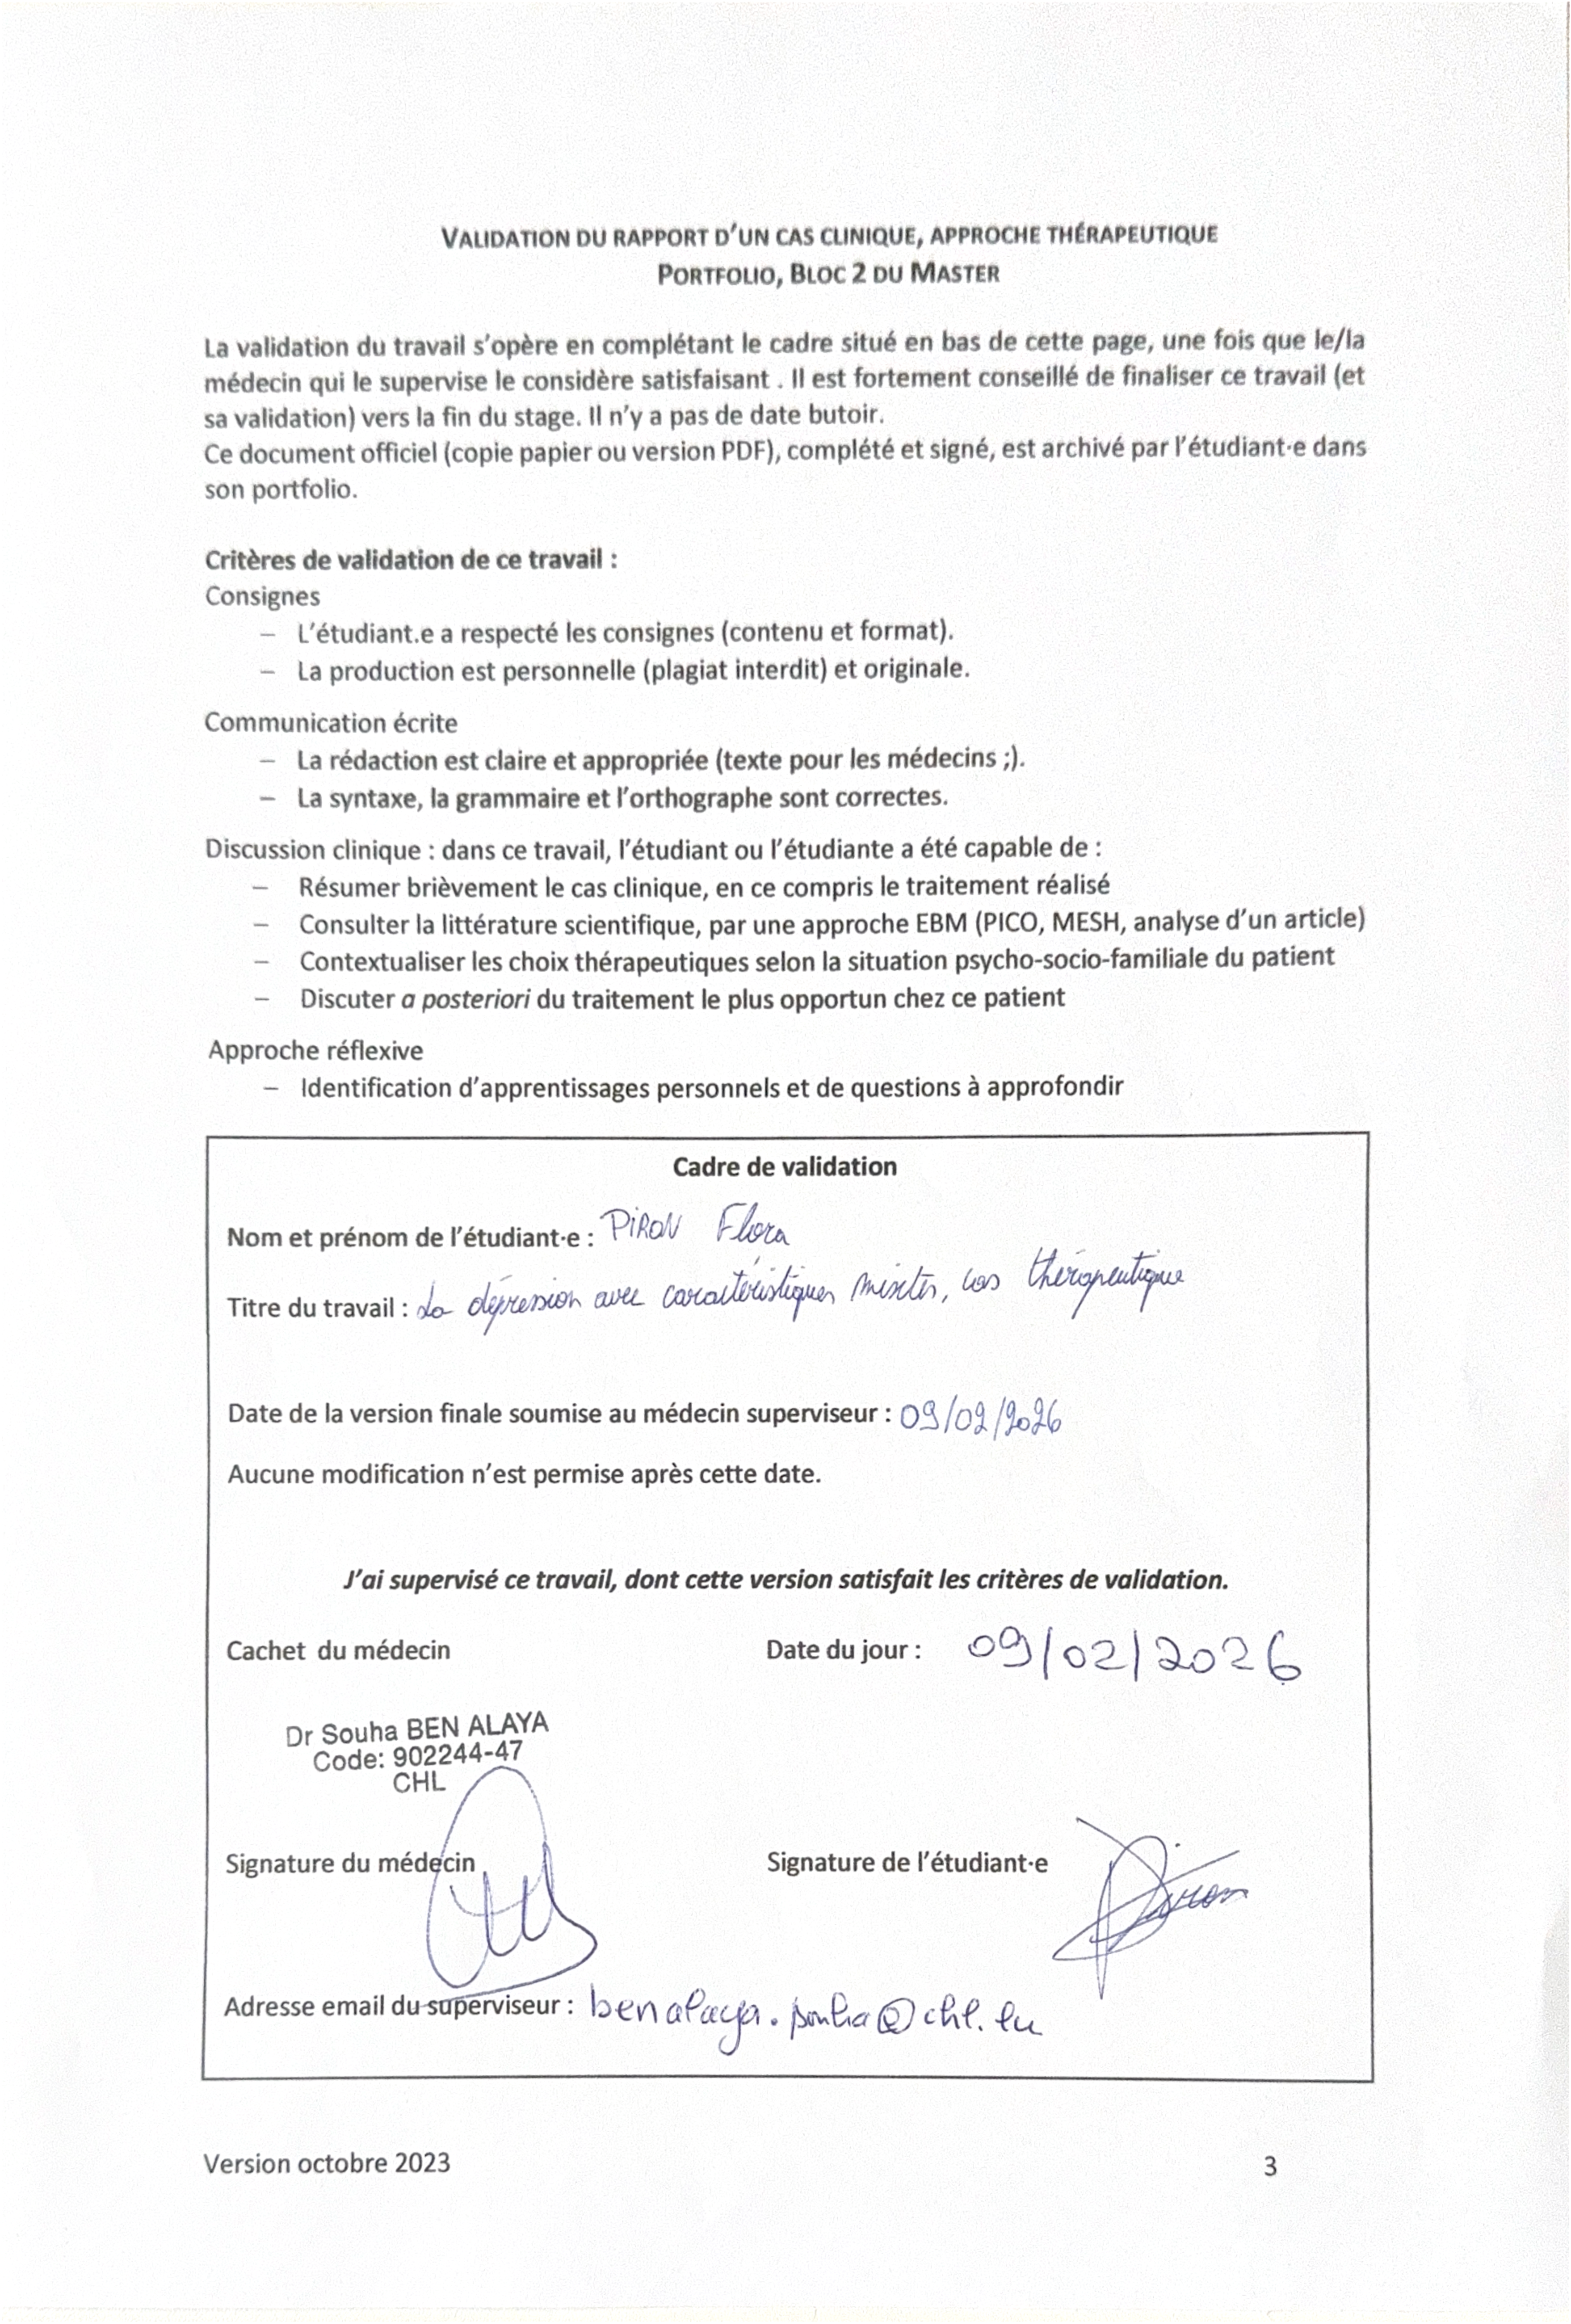
\includegraphics[width=0.9\textwidth]{figures/03-cas-therapeutique/Fiche_Validation_CasM2.pdf}
  \caption{fiche validation}
  \label{fig:fiche_validation_DrBenAlaya}
\end{figure}
\geometrieWord


\includepdf[pages=1, pagecommand={\thispagestyle{empty}}]{figures/covers/FP_Page_de_garde_page_05.pdf}


\chapter{Incident médical}

\section{Description de l'incident}

Un patient est né dans un contexte de déni de grossesse jusqu’à l’accouchement dans un hôpital à \qty{40}{\SA}. En effet, la maman en devenir s’est présentée aux urgences pour maux de dos. Suite à cela, l’accouchement a eu lieu. Retour à domicile du patient et de sa famille tel un accouchement classique au bout de 4 jours, sans procédure supplémentaire.

Dans le cadre de son suivi pédiatrique, l’enfant a été vu pour son vaccin des 2 mois. A ce moment, une hypotonie et une perte de poids importante sont mises en évidence : poids de naissance est de \qty{4.060}{\kg}, lors du premier mois de vie, il y a une prise de \qty{50}{\g} puis une perte de \qty{500}{\g}. Une hospitalisation aux soins intensifs est mise en place. A la sortie des soins intensifs 16 jours plus tard, l’enfant pèse \qty{4.545}{\kg}. En parallèle, une évaluation sociale est en cours car une dénutrition par manque d’apport est évoquée. Ensuite, l’enfant est transféré et poursuit son hospitalisation durant \qty{48}{\hour} vu la bonne prise de poids observée. De plus, l’équipe médicale s’intéresse au contexte familial au sens large car le patient a une fratrie, nous tentons donc d’assurer la bonne santé de ces enfants. Un signalement pour la protection de l’enfant est considéré mais n’est pas appliqué. Selon l’équipe multidisciplinaire, une chance supplémentaire est donnée à ces parents vu le contexte de déni de grossesse et un deuil du côté maternel qui s’est additionné à la situation sociale lors du premier mois de vie du patient. Des aides dans le quotidien de cette famille et un suivi rapproché sont également mis en place.

Deux semaines plus tard, une consultation post-hospitalisation est programmée. A nouveau une perte de poids est observée. L’enfant est à nouveau hospitalisé pour dénutrition sévère. Une fois l’alimentation recontrôlée par les soignants, l’enfant reprend du poids. En outre, lors de l’hospitalisation, aucun lien d’attachement n’est observé entre la maman et le patient. La maman ne porte que peu d’attention à celui-ci et elle garde une expression neutre tout au long de l’hospitalisation même lorsque nous évoquons la gravité de la situation. Un signalement pour protection de l’enfance est mis en place et approuvé par la Juge responsable du cas. S’en suit le retrait de la garde de l’enfant par la Police.

L’enfant poursuit donc son hospitalisation sous la garde de l’hôpital et une prise de poids est toujours observée. Les parents expriment de l’incompréhension et défendent qu’ils prennent soin de leur enfant attribuant la perte de poids sévère à la présence d’adénovirus dans les selles du patient. Or, l’équipe médicale est formelle que celui-ci ne peut être responsable à lui seul de cette chute de poids drastique. Cependant, un bilan complémentaire afin d’exclure tout autre diagnostic pouvant expliquer la situation est en cours. L’avenir de cet enfant reste incertain à ce jour, sera-t-il placé en foyer ou en famille d’accueil ? Aura-t-il encore des contacts avec ses parents ? Son état général et son hypotonie vont-ils se résoudre ? Qu’en deviendra-t-il de la fratrie ? Un suivi psychologique/ psychiatrique sera-t-il organisé pour la maman ? 

\section{Implications éthiques, déontologiques et légales de l’incident }

La problématique qui m’interpelle d’emblée est le manque de prise en charge lors de la naissance de l’enfant. Suivre le protocole de naissance classique ne me semble pas adapté à la situation. La physiopathologie du déni de grossesse n’est pas encore élucidée entièrement à ce jour mais il est bien connu qu’il est le reflet d’un traumatisme chez la maman. De plus, le déni de grossesse total, c’est-à-dire jusqu’à l’accouchement, représente un facteur de risque du passage à l’acte et la maltraitance de l’enfant. L’accouchement est un bouleversement psychologique intense pour la maman. Elle se présente aux urgences, dans ce cas pour des lombalgies puis se retrouve engagée dans un travail  en vue d’une naissance. L’enfant n’est pas attendu, aucune relation n’a été créée lors de la grossesse, la femme n’a pas eu l’occasion de devenir mère comme l’explique Sophie Marinopoulos dans \textcite{marinopoulos_deni_2019}. A la naissance du patient, il y a un manquement clair au niveau de plusieurs principes de la Bioéthique selon Beauchamp et Childress. D’une part la bienfaisance vis-à-vis de l’enfant a été négligée vu les facteurs de risque de négligence et la prévention d’un point de vue médical qui était possible. D’autre part, la bienfaisance vis-à-vis de la mère. Le déni de grossesse montrant clairement une souffrance psychique qui aurait dû être explorée par un professionnel de santé formé.

\todoH[GuillaumeVertStyle][green!25]{Bibliographie Lagedamon et al. (2025) : vérifier et compléter le prénom manquant pour l'auteur Baraille dans \emph{references.bib}.}{Une revue de la littérature},  \textcite{lagedamon2025accompagnement} appuie une fois de plus l’intérêt de prendre en charge la maman qui a souffert d’un déni de grossesse. Un protocole standardisé afin de prendre en charge le déni de grossesse manque cruellement ce qui a pour conséquence des prises en charge hétérogènes voire inexistantes. Or, un suivi psychologique pour la maman qui a un risque augmenté de stress post-traumatique ou dépression post partum, a montré des bénéfices. Les psychothérapies telles que EMDR, \textit{Eye Movement Desensitization and Reprocessing}, peuvent permettre une amélioration clinique de la maman. Ensuite, l’établissement d’un lien d’attachement avec son enfant est envisageable et peut permettre de prévenir les situations de négligence voire les néonaticides qui sont certes rares mais extrêmement graves.

Je remets également en question le respect du principe de la justice dans ce contexte. Autrement appelé l’équité, la justice consiste à traiter chaque personne de façon loyale, équitable et appropriée en fonction de ses spécificités. L’enfant a le droit d’avoir les mêmes chances de s’épanouir malgré un contexte de déni de grossesse et un milieu défavorisé. Est-il réellement éthique de ne pas avoir mis en place des aides autours de la famille afin de compenser l’environnement de l’enfant au moment de sa naissance ?

Je pourrais également ajouter à ce principe de justice comment peut-on demander à des parents ayant vécu un déni de grossesse total d’élever leur enfant comme une naissance classique sans outils, sans aide extérieure ?

Ce cas clinique met en lumière toute la complexité du signalement pour la protection de l’enfant dans un cadre de maltraitance. Le placement d’enfant soulève de nombreux défis éthiques. Le conflit entre la bienfaisance et la non-malfaisance est au centre du dilemme éthique. D’une part, la priorité est le bien-être de l’enfant voire la survie de celui-ci. Son passage en réanimation témoigne de l’urgence de la situation. La cassure de courbe de ce patient a été le point d’appel pour établir le diagnostic de malnutrition par manque d’apport. En effet, après la mise en évidence des facteurs de risque prédisposant à la maltraitance tel que l’état psychologique de la mère, le contexte de déni de grossesse, la situation financière de la famille, les connaissances des parents à propos du développement de l’enfant,…  les pédiatres responsables devaient évoquer la maltraitance comme expliqué dans ce clinical report \textcite{block2005failure}. De plus, la déontologie appuie d’autant plus le principe de bienfaisance. L’article 61 du code de Déontologie Médicale belge stipule que « \textit{Si la situation le justifie, et pour autant que la personne vulnérable capable de discernement y consente, le médecin s'adressera à un confrère compétent en la matière ou fera appel à une structure pluridisciplinaire spécifiquement établie pour gérer cette problématique. Si la personne vulnérable est menacée par un danger grave et imminent ou s'il y a des indices graves d'un danger sérieux et réel que d'autres personnes vulnérables soient victimes de maltraitance ou négligence et que le médecin n'a pas d'autre moyen d'offrir une protection, il peut avertir le procureur du Roi de ses constatations }». Suite à l’échec de la mise en place d’aide au domicile, une stratégie de non malfaisance dans le but de conserver la relation thérapeutique avec les parents, le signalement fut une solution envisageable pour l’ensemble de l’équipe médicale.

L’aspect légal intervient également dans la prise de décision du placement de l’enfant. La loi qui doit être prise en compte dans cette situation. Selon l'article 15, §~2 de la loi du 22 août 2002 relative aux droits du patient, le médecin a le droit de déroger à la décision des parents (ou du représentant légal) si celle-ci met en danger la vie de l'enfant ou constitue une atteinte grave à sa santé. Donc, en considérant l’aspect légal, le corps médical a l’obligation de faire ce signalement dans l’immédiat afin d’assurer la survie du patient.

Toutefois, le principe de non-malfaisance doit être exploré dans cette situation. En effet, est-ce que le placement de l’enfant est la meilleure solution pour lui et son développement ? Il est démontré dans cette étude \textcite{poitras2017contacts} que le placement des jeunes enfants réduit la probabilité de réunification avec les parents biologiques et une stabilité de trajectoire. Selon eux, la stabilité de la trajectoire se définit par trois critères : les tentatives de réunification familiale, l’échec de la réunification et le nombre d’hébergements qu’a vécus l’enfant. Toutefois, plusieurs limites se retrouvent dans cette étude dont un échantillon de petite taille ce qui empêche de pouvoir interpréter les résultats avec certitude. Cependant, cette étude confirme également les résultats obtenus dans la littérature scientifique. Peut-on extrapoler cette instabilité de trajectoire comme représentation objective du malheur de l’enfant ou en tout cas d’une mauvaise prise en charge au final ?

Par contre, une autre étude, \textcite{mascaro2012evaluation} démontre l’importance d’apporter l’attention, la stimulation psychique et physique du nourrisson durant cette période critique. Sans cette attention, l’enfant peut développer un trouble important du développement d’où l’importance de sortir l’enfant de cet environnement négligent. La pouponnière peut être une option, si et seulement si elle peut assurer une prise en charge constante et régulière. Donc, la décision entre séparer l’enfant de sa famille et le placer dans une famille d’accueil ou une pouponnière est bien sûr à nuancer et comparer les soins qui sont possibles et à quelle fréquence concrètement ils peuvent être réalisés. Une autre remarque reprise dans cet article est l’importance de la persévérance. Celui-ci n’a effectué un suivi que sur 4 mois mais déjà dans ce délai, ils ont observé un rythme différent chez plusieurs enfants. Cela signifie donc, que le soignant responsable de l’enfant ne doit pas perdre espoir une fois les soins mis en place car des améliorations voire une reprise du développement physiologique est possible. Le dilemme éthique et la balance pour ou contre le placement de l’enfant n’est pas univoque, il s’agit d’un équilibre fragile.

En conclusion, le plus grand problème éthique que j’ai identifié dans cette situation clinique est le manque de prise en charge à la naissance du patient. Un autre aspect éthiquement intéressant est tout la complexité du placement de l’enfant pour sa survie et son bon développement ainsi que les alternatives de prises en charge possible pour l’enfant et le déni de grossesse de la maman.

\section{Conduite à tenir selon l’étudiante }

Différents scénarios sont envisageables mais selon moi, le scénario le plus éthique aurait été une prise en charge multidisciplinaire dès la naissance du patient et la découverte du déni de grossesse. Une prise en charge psychologique voire psychiatrique selon le contexte, me parait obligatoire pour prévenir toute maltraitance et trouble dans la relation mère-enfant ainsi que de désamorcer la culpabilité que la maman ressentira. Prolonger l’hospitalisation lors de la naissance jusqu’à observer un attachement entre l’enfant et la mère ou tout signe qui va en ce sens afin d’avoir l’assurance nécessaire pour permettre un retour à domicile me parais indispensable. La suite du plan thérapeutique comprendrait une mise en place des aides dans le quotidien de la famille et en plus, être attentif en tant que médecin au deuil que la maman a traversé lors des premières semaines de vie du patient. Je pense que cette prise en charge aurait pu prévenir le passage en réanimation. Sans même transformer trop les faits et idéaliser la psychothérapie, la surveillance extérieure de cette famille, avec un regard bienveillant et médical aurait permis de dépister la dénutrition plus précocement. Avec cette présence du monde médical, cela permet de gagner du temps et laisser l’opportunité d’aborder l’approche centrée sur le patient.

Apporter cependant une nuance à ce scénario utopique est primordial car la condition nécessaire pour que cela fonctionne est que les parents acceptent la prise en charge et la présence de l’équipe soignante dans leur quotidien. A nouveau, avec une approche centrée sur le patient, les soignants ne s’imposent pas aux patients donc je reste convaincue qu’avec une communication adaptée une relation thérapeutique peut être entretenue. Il est important de notifier également que les parents se sont présentés à plusieurs consultations médicales prévues ce qui montre une collaboration fragile mais présente. Sans doute, ceci est une porte d’entrée pour un travail ensemble dans l’intérêt du patient.

\todoH[FloraStyle][red!30]{pe mettre ce lien en note bas de page parce que ça m'a inspiré pour trouver une conduite en plus à faire \url{https://www.yapaka.be/sites/yapaka.be/files/texte/15_06_19_le_deni_de_grossesse-a_mettre_en_ligne_0.pdf}}{Le professionnel de santé} a bien sûr son rôle à jouer dans la reconnaissance de la grossesse le plus tôt possible afin d’éviter un déni de grossesse total. Au-delà du diagnostic précoce qui permet de limiter les complications, il est simplement important que le médecin reconnaisse le phénomène et la déconstruction des croyances qui entourent le déni de grossesse. Éviter le tabou de celui-ci permet une meilleure prise en charge et éviter la dénutrition sévère par carence d’apport. Des protocoles standardisés pour encadrer la prise en charge du déni de grossesse permettent de limiter les erreurs individuelles de chaque médecin et d’uniformiser les connaissances. La rédaction de ces protocoles serait l’idéal et une des premières idées qui vient en tête. Toutefois, si je dois rester réaliste, je dois considérer la difficulté que cela représente de mener des études cliniques et pouvoir tirer des conclusions statistiquement significatives avec un échantillon aussi réduit et ainsi pouvoir élaborer des guidelines pertinentes.

Pour conclure ce cas clinique, je pense que la prise en charge réelle n’a pas été optimale et surtout aurait pu être différente à plusieurs niveaux. Cependant, je pense qu’il est toujours plus simple de réfléchir au cas clinique a posteriori, sans urgence et avec du recul sur l’évolution de la situation. La prise de décision est toujours influencée par de nombreux facteurs et parfois, certains arguments prennent plus de poids qu’ils ne devraient ce qui entraine des conséquences néfastes. Pour ce patient, la suite de son histoire a été tragique mais grâce à plusieurs garde-fous, l’enfant a survécu et l’espoir d’une amélioration de son développement est toujours possible.

\section{Approche réflexive}
\subsection{Les connaissances/compétences acquises lors de la rédaction de cet incident clinique ;}
\begin{itemize}[label=\textbullet]
    \item Approfondir ma capacité de recherche dans la littérature car celle-ci était pauvre pour cette thématique. Rechercher de nouvelles bases de données et aiguiser d’autant plus mon esprit critique.
    \item La déconstruction sur certaines croyances vis-à-vis du déni de grossesse. J’ai eu l’occasion de développer la physiopathologie et d’améliorer la façon dont je souhaitais aborder les patientes expérimentant un déni. 
    \item Ce cas clinique a montré l’importance de la pluridisciplinarité. Au-delà de l’équipe soignante, il y avait une collaboration étroite avec l’assistante sociale et avec la Juge responsable. L’aspect social étant vraiment présent et imbriqué dans la santé et la clinique du patient que l’assistant social devient un membre primordial et fait partie intégrante de la prise en charge. 
    \item Observer de mes yeux l’absence de lien mère-enfant a provoqué en moi beaucoup d’émotions et d’incompréhension. Il m’a fallu apprendre à prendre du recul sur la situation et garder un professionnalisme sans laisser transparaître mes sentiments et moi-même me protéger de cet impact.
\end{itemize}

\subsection{Les influences probables de ce travail sur sa pratique médicale future ;}

\begin{itemize}[label=\textbullet]
    \item Ne pas stigmatiser les patients selon leur milieu social et prendre le temps de comprendre la problématique et le contexte. Celui-ci peut aider à la prise en charge et savoir comment communiquer et établir une relation de confiance avec le patient et sa famille.
    \item Préserver la curiosité d’en apprendre plus sur les pathologies que l’on rencontre en clinique. Se remettre en question sur les bases acquises et rester à jour au niveau du savoir médical.
\end{itemize}

\subsection{Les difficultés (dépendantes ou indépendantes de sa volonté) ayant entravé son acquisition de nouvelles connaissances/compétences au cours de cette expérience ;}

\begin{itemize}[label=\textbullet]
    \item La restriction de l’information contenue dans les protocoles ou rapport présent dans le dossier. Les anamnèses d’entrée sont clairement centrées sur la clinique, toutefois, vu le contexte, avoir davantage d’informations sur l’aspect social aurait été utile.
    \item En lien avec l’émotion ressentie, j’ai également ressenti beaucoup d’impuissance. Je pense qu’il est naturel d’avoir un réflexe correcteur face à ce patient si jeune qui subit beaucoup face à un environnement nuisible. Je peux ajouter que face au déni des parents, il était parfois difficile de trouver mes mots afin de rester professionnel et d’avoir les termes appropriés et juste dans le sens que e-je voulais leur donner.
\end{itemize}

\subsection{Les solutions que l’étudiant·e peut mettre en place pour remédier à ces difficultés.}

\begin{itemize}[label=\textbullet]
    \item Pour améliorer les rapports, je peux penser à ajouter de façon systématique un contexte social et détailler les circonstances d’admission. 
    \item Il est important de déconstruire ce réflexe qui parfois entrave la bonne prise en charge et la relation thérapeutique. Le premier pas est d’abord de le reconnaitre et d’en prendre conscience. Ensuite, si le besoin en est, communiquer de cette problématique à un collègue voire à un professionnel afin d’être accompagné dans cette démarche. Plusieurs ouvrages existent et aident le soignant qui prend la peine de les lire. 
    \item D’un point de vue purement communicationnel, je pense qu’il me reste beaucoup à apprendre et la formation peut-être multimodal via des cours, des ouvrages, des conférences,…
    \end{itemize}




\chapter{Cas Polypathologique complexe}

\section{Rapport synthétique}

\subsection{Cas clinique}
Patient de $79$ ans est hospitalisé pour décompensation cardiaque avec fraction d’éjection conservée à $66$\%, Heart Failure with preserved Ejection Fraction (HFpEF) à la suite de l’administration de la première dose d’Azacitidine (Vidaza). Azacitidine est un agent déméthylant de l’ADN prescrit dans le cadre d’une leucémie myéloïde aiguë.

Antécédents médicaux pertinents

\begin{itemize}[label=\textbullet]
    \item Diabète de type $2$ ;
    \item Syndrome métabolique ;
    \item Cardiopathie hypertensive avec dysfonction diastolique \todoH[FloraStyle][red!30]{\ !!! faut savoir c'est quoi la classification !}{\mbox{franche de grade $2$}} ;
    \item Dermo-hypodermite au niveau prétibial gauche ;
    \item Fibrillation atriale ;
    \item Infarctus du myocarde 
    \item BPCO GOLD II
    \item Leucémie myéloïde aiguë
    \end{itemize}

Antécédents chirurgicaux pertinents

\begin{itemize}[label=\textbullet]
    \item Mise en place d’un Pacemaker DDD ;
    \end{itemize}

Allergies et assuétudes

\begin{itemize}[label=\textbullet]
    \item Pas d’allergie connue à ce jour ;
    \item Tabac : $50$ UPA ($2$ paquets/j pendant $25$ ans) arrêté depuis une vingtaine d’années ;
    \item Alcool : occasionnelle ;
    \item Il nie toute autre consommation ;
    \end{itemize}


Médication (en septembre $2026$) reprise dans le~\cref{tab:medication_patient}.

% ====================================================================================
% VERSION 3 : PAYSAGE / PENCHÉ (STYLE LES_HYPOTHESES_DIAGNOSTIQUES)
% Page pivotée automatiquement dans le visualiseur PDF avec grille complète (| et \hline)
% ====================================================================================
\begin{landscape}
\begingroup
\footnotesize
\setlength{\tabcolsep}{5pt}
\renewcommand{\arraystretch}{1.05}

\begin{xltabular}{\linewidth}{|>{\raggedright\arraybackslash\bfseries}p{4.2cm}|>{\raggedright\arraybackslash}p{3.6cm}|>{\raggedright\arraybackslash}p{5.8cm}|>{\raggedright\arraybackslash}X|}
    \caption{Médication du patient (septembre 2026)} \label{tab:medication_patient} \\
    \hline
    \rowcolor{gray!15}
    \textbf{DCI} & \textbf{Nom commercial \& Posologie} & \textbf{Classe pharmacothérapeutique} & \textbf{Indication clinique} \\
    \hline
    \endfirsthead

    \caption*{Tableau~\ref{tab:medication_patient} (suite) -- Médication du patient (septembre 2026)} \\
    \hline
    \rowcolor{gray!15}
    \textbf{DCI} & \textbf{Nom commercial \& Posologie} & \textbf{Classe pharmacothérapeutique} & \textbf{Indication clinique} \\
    \hline
    \endhead

    \hline
    \multicolumn{4}{|r|}{\footnotesize\textit{Suite du tableau à la page suivante...}} \\
    \hline
    \endfoot

    \hline
    \endlastfoot

    Ézétimibe / Atorvastatine & 
    Atozet \qty{10}{\mg} / \qty{40}{\mg} \newline 1 cp/j & 
    Hypolipémiant combiné (inhibiteur sélectif de l'absorption du cholestérol + statine de haute intensité) & 
    Prévention cardiovasculaire secondaire. \\
    \hline

    Bumétanide & 
    Burinex \qty{1}{\mg} \newline 1 cp/j & 
    Diurétique de l'anse de Henle & 
    Traitement déplétif de la surcharge hydrosodée : contrôle des pressions de remplissage ventriculaire gauche élevées liées à la cardiopathie hypertensive avec dysfonction diastolique de grade 2. \\
    \hline

    Bisoprolol & 
    Bisoprolol \qty{10}{\mg} \newline ½ cp/j (\qty{5}{\mg}/j) & 
    Bêtabloquant $\beta_1$ cardiosélectif & 
    Cardiopathie hypertensive \& contrôle hémodynamique : baisse des résistances vasculaires périphériques, allongement du temps de remplissage diastolique par ralentissement de la fréquence cardiaque, et freinage de l'hyperactivité sympathique. \\
    \hline

    Amiodarone & 
    Cordarone \qty{200}{\mg} \newline 1 cp/j & 
    Antiarythmique de classe III de Vaughan-Williams & 
    Prévention des récidives de tachyarythmie supraventriculaire. \\
    \hline

    Fluticasone furoate / Uméclidinium / Vilantérol & 
    Trelegy Ellipta 92/55/22\,\unit{\ug} \newline 1 inh/j & 
    Trithérapie inhalée fixe : Corticoïde inhalé (CSI) + Anticholinergique à longue durée d'action (LAMA) + $\beta_2$-mimétique à longue durée d'action (LABA) & 
    Traitement de fond de la BPCO. \\
    \hline

    Bromure d'ipratropium / Fénotérol & 
    Duovent \newline (posologie à la demande) & 
    Bronchodilatateur d'action rapide combiné : Anticholinergique à courte durée d'action (SAMA) + $\beta_2$-mimétique à courte durée d'action (SABA) & 
    Traitement de secours / à la demande : levée immédiate du bronchospasme et prise en charge des accès dyspnéiques paroxystiques dans la BPCO. \\
    \hline

    Apixaban & 
    Eliquis \qty{5}{\mg} \newline 1 cp 2$\times$/j & 
    Anticoagulant oral direct (AOD) & 
    Thromboprophylaxie systémique liée à l'arythmie supraventriculaire associée (score $\mathrm{CHA_2DS_2}\text{-}\mathrm{VA}$ élevé). \\
    \hline

    Cholécalciférol (Vitamine $\mathrm{D_3}$) & 
    Vista $\mathrm{D_3}$ \newline 1 cp/j & 
    Vitamine D / régulateur du métabolisme phosphocalcique & 
    Prévention de l'ostéopénie / ostéoporose. \\
    \hline

    Zolpidem & 
    Stilnox \qty{10}{\mg} \newline 1 cp le soir & 
    Hypnotique apparenté aux benzodiazépines & 
    Traitement symptomatique de courte durée de l'insomnie d'endormissement. \\
    \hline

    Azacitidine & 
    Vidaza \newline Cure palliative par voie sous-cutanée : 7 jours/mois pendant 28 jours & 
    Agent déméthylant de l'ADN & 
    Traitement de la leucémie myéloïde aiguë non éligible à une chimiothérapie d'induction intensive. \\
    \hline

    Dapagliflozine & 
    Forxiga \qty{10}{\mg} \newline 1 cp/j & 
    Inhibiteur du cotransporteur sodium-glucose de type 2 (iSGLT2) & 
    Triple indication : \newline
    \textbullet~Diabète de type 2 ; \newline
    \textbullet~Cardioprotection ; \newline
    \textbullet~Néphroprotection. \\
    \hline

    Oxygénothérapie chronique & 
    \qty{2}{\L\per\minute} par oxyconcentrateur & 
    Support ventilatoire & 
    Support pour l'hypoxémie nocturne et les troubles de diffusion dans le cadre de la BPCO. \\
\end{xltabular}
\endgroup
\end{landscape}


Contexte psyho social : 
Le patient vit au domicile avec son épouse. Elle est très présente pour le patient. Le patient a $2$ enfants et $4$ petits-enfants. 
Le patient se sent très limité, dyspnéique et trouve le temps long en chambre.  Une thymie triste domine dans le discours du patient. 

Histoire clinique :

Le patient est hospitalisé dans le service d’onco-hématologie pour insuffisance respiratoire de type I sur décompensation cardiaque. Suite à l’administration de la première dose d’Azacitidine (Vidaza) dans le contexte de sa leucémie myéloïde aiguë, le patient a présenté une dyspnée de grade IV NYHA évolutive avec sensation d’oppression thoracique. Ceci s’ajoutant à des signes cliniques caractéristiques de la décompensation cardiaque décrits dans l’examen clinique. Il a été décrit dans la littérature une augmentation significative d’événement cardio-pulmonaire lorsque le patient a des polymorbidités de ces systèmes. De plus, la dyspnée est répertoriée comme un effet indésirable très fréquent selon \textcite{ema_azacitidine_accord}.

Paramètres d’entrée :
\begin{itemize}[label=\textbullet]
    \item Tension artérielle couché : $96/70$
    \item Saturation : $91$\% sous $4$L/min d’oxygène
    \item Température : $36,8$°C
    \item Pouls : $69$/min
    \item Taille : $167$cm
    \item Poids : $58$kg
    \item BMI : $20,8$ kg/m$^2$
    \end{itemize}

Examen clinique d’entrée :
    \begin{itemize}[label=\textbullet]
    \item Apparence : pâle.
    \item Examen neurologique : le patient est orienté dans l’espace et le temps. Score de Glasgow de $15/15$.
    \item Examen pulmonaire : eupnéique sous 4L/min d’oxygène. A l’auscultation, murmure vésiculaire diffus et symétrique sans sibilance. Crépitants bibasilaires entendus.
    \item Examen cardiaque et vasculaire : les jugulaires sont turgescentes avec un reflux hépato-jugulaire. Présence d’œdème des membres inférieurs de façon bilatérale avec prise du Godet à la palpation. A l’auscultation, B$1$B$2$ réguliers. Pas de souffle ni galop.
    \item Examen abdominal : péristaltisme normal à l’auscultation. Abdomen souple, dépressible, légèrement sensible en fosse iliaque gauche à la palpation. Pas d’organomégalie palpée.
    \end{itemize}


\subsection{Prise en charge hospitalière}
Volet cardio-pneumologique : 
\begin{itemize}[label=\textbullet]
    \item \underLine{A l’admission} : présentation clinique d’une décompensation cardiaque claire. Notamment des signes de décompensation cardiaque droite avec des œdèmes des membres inférieurs prenant le Godet, des jugulaires saillantes et un reflux hépato-jugulaire ainsi que des signes d’une décompensation cardiaque gauche avec des crépitants bibasilaires à l’auscultation. De plus, la biologie appuie cette étiologie avec un dosage de NT Pro-BNP à $2055.0$ pg/mL et la radiographie de thorax a démontré une cardiomégalie modérée avec surcharge vasculaire hilaire gauche.
    \item  \underLine{Avis cardiologique requis} : suite à la réalisation d’une échographie cardiaque, nous pouvons conclure que la fonction ventriculaire gauche est conservée et la dynamique régionale normale. Absence, donc, d’argument en faveur d’une élévation des pressions de remplissage. Par contre, une insuffisance tricuspidienne modérée et une hypertension artérielle pulmonaire est démontrée. Le cardiologue préconise une administration de Lasix IV et augmentation des doses du  Bumétanide  à $2,5$mg en conservant le Dapagliflozine. Une augmentation de l’oxygénothérapie à $4$L/min est proposée, à adapter selon la clinique et les paramètres du patient au cours de l’hospitalisation.
    \item \underLine{ Épisode de désaturation à $80$\% sous $3$L/min d’oxygène $4$ jours après l’admission} : augmentation de l’oxygénothérapie à $5$L/min a permis une saturation à $87$\%. Dans les heures qui ont suivi, le débit a pu redescendre à $3,5$L/min. Un nouveau bilan est débuté comprenant une radiographie du thorax, une biologie et un ECG. Les résultats principaux sont une majoration de l’infiltrat interstitiel bilatéral sur lésions de broncho-emphysème diffus sans foyer parenchymateux systématisé, une biologie avec D-Dimère à $750$ ng/mL, GOT $145$ U/L, proBNP $13 000$ pg/mL, Troponine $0,025$ µg/L à interpréter dans le contexte global de décompensation cardiaque, à savoir qu’il n’y avait aucune douleur thoracique rapportée. Une aérosolthérapie par Duovent a été débutée ainsi qu’une majoration du Bumétanide d’$1$mg et une ampoule de $0,5$mg de morphine qui a soulagé la symptomatologie. Bien que l'avis cardiologique ait suspecté une cause respiratoire prédominante (surinfection à Pseudomonas), l'ascension majeure du NT-proBNP à $13 000$ pg/mL et la réponse à la majoration du Burinex signent un tableau mixte. 
\end{itemize}

Volet infectiologique : 
\begin{itemize}[label=\textbullet]
    \item \underLine{Au cours de l’hospitalisation} : Monsieur présentait des expectorations purulentes avec péjoration de la dyspnée et une altération de l’état général. Toutefois, le patient est resté apyrétique durant l’ensemble de l’hospitalisation.
    \item \underLine{Avis infectiologique} : une surinfection pulmonaire a été suspectée. Il a été décidé de couvrir le patient par amoxicilline / acide clavulanique selon une antibiothérapie probabiliste. Cependant, à la suite de la positivité à Pseudomonas aeruginosa, bacille pyocyanique, la ceftazidime a été initiée pendant 7 jours.
    \end{itemize}

Volet Hémato-oncologique :
\begin{itemize}[label=\textbullet]
    \item \underLine{A l’admission} : interruption du traitement d’Azacitidine suite au contexte cardio-pulmonaire. 
    \item \underLine{Lors de l’hospitalisation} : surveillance étroite des marqueurs hématologiques. Une neutropénie débutante secondaire à Azacitidine a été observée.
    \item \underLine{A la sortie} : planification des soins et la poursuite du traitement palliatif de la leucémie myéloïde aiguë.
    \end{itemize}


Les équipes pluridisciplinaires intervenant au cours de l’hospitalisation de Monsieur :
\begin{itemize}[label=\textbullet]
    \item \underLine{L’équipe infirmière/aide-soignant} au cœur des soins. Le rôle majeur est dans la surveillance constante du patient et la transmission d’informations pertinentes à l’équipe médicale. Les infirmiers ont aussi l’opportunité de stimuler le patient à se mettre au fauteuil et apporter l’aide quotidienne nécessaire au patient. 
    \item \underLine{La diététicienne}  est intervenue dans ce cas, suite aux signes de fausses déglutitions rapportées par le patient et l’équipe infirmière. Les textures alimentaires ont pu être adaptées afin de correspondre aux besoins de Monsieur.
    \item \underLine{L’équipe des soins continus/palliatif et l’équipe sociale} ont collaboré ensemble afin de conclure à une solution envisageable par la patient et ses proches pour la suite de la prise en charge. Les conditions du projet thérapeutique ont également été rediscutées lors de l’hospitalisation afin de préserver la collaboration avec Monsieur et s’assurer une qualité de soins. 
    \item \underLine{Le psychologue de liaison} n’a pas été sollicité par refus du patient.
    \end{itemize}
    
Voir détails des examens complémentaires en \cref{annexe:examens_complementaires} en \cpageref{annexe:examens_complementaires}.

\subsection{Complexités rencontrées}
\begin{itemize}[label=\textbullet]
    \item \underLine{Complexité diagnostique} : déterminer l’étiologie de la dyspnée parmi un tableau clinique complexe. La multitude de pathologies que le patient cumule sont réparties dans les différents systèmes. Devoir agir dans l’urgence et décider un traitement est complexe.
    \item \underLine{Complexité thérapeutique} : aborder un patient avec autant de traitements concomitants est difficile et requiert une précaution supérieure face aux interactions médicamenteuses possibles. Savoir élaguer la liste médicamenteuse afin de garantir le plus de confort au patient est une tâche complexe.
    \item \underLine{Complexité psycho-sociale} : la décision prise par le patient ne correspond pas forcément à la solution idéale au niveau médical. Il faut donc apprendre à accepter l’autre et passer au-dessus de ce sentiment de frustration qui peut survenir.
    \end{itemize}
\subsection{Éclairage d’un aspect thérapeutique}
\subsubsection{Méthode}
\underLine{Formulation de la question clinique selon la méthode PICO :}
\begin{itemize}[label=\textbullet]
    \item POPULATION : patient polypathologique âgé atteint d'insuffisance cardiaque à fraction d'éjection préservée (HFpEF, FE $66$ \%) et diabète de type $2$.
    \item INTERVENTION : administration d'un inhibiteur du SGLT$2$.
    \item COMPARATEUR : traitement conventionnel sans iSGLT$2$ / placebo.
    \item OUTCOME : réduction des réhospitalisations pour décompensation cardiaque, mortalité et amélioration de la qualité de vie.
    \end{itemize}
\underLine{Base de données consultée :} PubMed.\\
\underLine{Equation de recherche utilisée :} ("Sodium-Glucose Transporter $2$ Inhibitors"[Mesh] OR "dapaglifloxzin") AND ("HFpEF"OR "preserved ejection fraction") AND ("Heart Failure"[Mesh] ).\\
\underLine{Critères de sélection :} date de publication <$5$ ans, texte intégral, revue systématique, méta-analyse.\\
\underLine{Date de consultation :} $25$ octobre $2026$.

\subsubsection{Résultat}
J’ai choisi la méta-analyse \textcite{minisy2025role}. Elle regroupe $9$ études randomisées entre $2015$ et $2025$ avec un ensemble de $20 000$ patients. La conclusion confirme l‘efficacité des inhibiteurs SGLT$2$ dans la prise en charge de l’insuffisance cardiaque avec fraction d’éjection préservée (HFpEF). La réduction du risque relatif de mortalité cardiovasculaire et le nombre d’hospitalisation pour insuffisance cardiaque serait de $17$\%. Ce résultat est obtenu de façon constante et significative à travers l’ensemble des études. Leur action sur la mortalité et la qualité de vie global tend à être favorable sans toutefois pouvoir être objectivée de façon significative. 

\subsubsection{Discussion}
Cette méta-analyse démontre clairement les bénéfices des inhibiteurs SGLT$2$ et donc justifie leur place au sein de la prise en charge de l’HFpEF. Plusieurs outils de qualités utilisés sont reconnus et validés tel que Cochrane RoB $2.0$, PRISMA $2020$ guidelines, évaluation GRADE, … ce qui est un avantage pour la méthode de l’analyse.

Toutefois, parmi les limites admises par les auteurs, nous retenons l’absence d’analyse en sous-groupe notamment pour dissocier les polymorbidités ou encore pour dissocier les différentes molécules utilisées. Ils l’expliquent par le choix de travailler sur des données agrégées et non individuelles. La définition stricte de la fraction d’éjection préservée n’a pas été respectée. Ils ont admis un plus faible pourcentage de fraction d’éjection allant jusqu’à $40$\% or en théorie, elle se limite à $50$\% ou plus. Au final, presque un tier de la cohorte a une fraction d’éjection <$50$\%. Le dernier point qu’ils mettent en lumière est l’hétérogénéité modérée au vu de l’ensemble des critères d’inclusion repris dans les différentes RCTs et les biais retrouvés dans certaines études notamment dû à un modèle non aveugle et aux données manquantes.

En analysant en détails la méta-analyse, j’ai pu remarquer d’autres défauts dans la conception de cette méta-analyse. D’une part, dans la sélection des RCTs, ils ont repris une étude, « DEFINE-HF » qui comprend dans son titre même « …...in patients with heart failure with reduced ejection fraction: DEFINE-HF trial » et certaines études, EMPEROR-Pooled et EMPEROR-Preserved, repris comprennent les mêmes patients et donc il s’agit d’un double comptage des patients ce qui fausse bien sûr les chiffres et l’importance des résultats obtenus. Un autre point primordial à aborder dans cette méta-analyse, spécifiquement lorsque la population est une population âgée, polypathologique, sont les effets indésirables et graves des inhibiteurs SGLT$2$. Or, cela n’a pas été analysé ou évoqué dans la méta-analyse.

En conclusion, il s’agit d’une méta-analyse ayant une base de données solide et une méthodologie de référence avec des outils fiables. Toutefois, plusieurs limites nous rappellent qu’il faut être vigilant quant à l’interprétation des résultats. Cependant, vu la tendance favorable des inhibiteurs SGLT$2$ sur le tableau clinique de l’insuffisance cardiaque à fraction préservée, il semble confirmer son rôle dans les guidelines. 

\subsubsection{Contextualisation} 
La décision médicale d’initier la bithérapie d’un diurétique de l’anse avec du Dapagliflozin dans le contexte de décompensation cardiaque était justifiée. De plus, cette méta-analyse appuie l’avis cardiologique donné à Monsieur, surtout vu la pertinence des outcomes tel que la réduction d’hospitalisation pour Monsieur désireux d’un projet de soins palliatifs à domicile.

Bien sûr, une surveillance clinique était requise compte tenu du nombre accru de médicaments et pathologies dont le patient souffrait afin de prévenir toute interaction médicamenteuse ou dégradation du patient. 
Un dilemme persiste en réalité car dans un contexte palliatif terminal où Monsieur était hypotendu à l’admission avec une alimentation pauvre, est-ce que finalement le Dapagliflozine avait-il sa place ? Bien sûr la réponse reste à nuancer et l’initiation de ce traitement était clairement justifiable au niveau médical. 

\subsection{Plan de soins proposé} 

Deux alternatives étaient réalisables pour Monsieur. D’une part, une place au sein de l’unité de soins palliatifs la plus proche de son domicile était disponible. L’ensemble de son traitement pouvait être assuré en ces lieux. D’autre part, un retour à domicile pouvait être envisageable en considérant la mise en place d’aide à domicile et d’une collaboration étroite avec l’équipe mobile de soins palliatifs « Accompagner».

La décision prise entre l’équipe soignante, son épouse et Monsieur a été le retour à domicile. Parmi les aides mises en place, notons le rôle central du médecin traitant qui a su être à l’écoute et se rendre flexible afin de répondre au mieux aux demandes du couple. In fine, un passage quotidien de l’équipe infirmière, les transports ou le matériel médical éventuellement prodigué par la Croix-Rouge ou son épouse elle-même pour assurer la continuité des traitements, les aides ménagères ou alimentaires sont également proposées. Un protocole de détresse a pu être élaboré en cas de dégradation du patient. Malheureusement, Monsieur décédera 6 jours plus tard au domicile toutefois paisiblement grâce aux soins apportés, un suivi de deuil est également organisé pour son épouse.

\subsection{Rôle en tant que stagiaire médecin} 

J’ai pu agir concrètement en mettant en contact l’équipe sociale avec le patient et ses proches. J’ai eu l’occasion d’interagir directement avec l’équipe des soins continus et palliatifs pour mieux comprendre les enjeux et les options réalisables pour monsieur et son épouse.

Étant stagiaire, je disposais de plus de temps pour être au chevet du patient. Cela m’a permis une communication plus authentique avec monsieur. Nous avons abordé ses peurs. J’ai tenté d’appliquer plusieurs techniques communicationnelles afin de matérialiser ses douleurs, réaliser l’origine réelle de celles-ci et surtout identifier les ressources possibles. Souvent, plusieurs choses peuvent être mises en place sans coût ni excès de temps or cela réconforte grandement le patient. Une différence peut être faite par la façon d’aborder le patient, les informations transmises et les explications claires et ciblées aux demandes du patient.  

 

\section{Approche réflexive}

\subsection{Les connaissances/compétences acquises grâce à la rédaction de ce cas clinique ;} 

En cours de cette hospitalisation, j’ai pu prendre le temps de comprendre en profondeur le dossier de monsieur. Rechercher les informations pertinentes parmi tous les comptes-rendus disponibles dans son dossier. Synthétiser un cas aussi complexe est déjà un exercice en lui-même.

De plus, vient s’ajouter l’aspect pharmacologique. Il faut comprendre la complexité des traitements médicamenteux et leur impact concret sur le patient et sa clinique. Remettre en question la légitimité de chaque molécule. Chez Monsieur, je suis convaincue que cette tâche n’a pas été exploitée dans son entièreté. Est-ce que la vitamine D et le traitement pour l’hypercholestérolémie avaient réellement leur place dans le pilulier de Monsieur vu le contexte palliatif ? Ou encore le Zolpidem, une Z-drogue que l’on doit remettre en question systématiquement vu l’usage abusif à long terme de cette classe de médicament. Son indication est à remettre en question  mais le sevrage n’est peut-être pas à envisager en aigu lors de son hospitalisation et dans le contexte des soins palliatifs.

\subsection{Les influences probables de ce travail sur sa pratique médicale future ;}

L’importance de clarifier le projet de soin et de façon précoce dans l’hospitalisation afin de prévenir une mauvaise gestion d’événement aigu. Au-delà de la connaissance médicale, notre rôle est d’aider le patient et de le soulager. Pour pratiquer de la bonne médecine, il faut être en accord avec le patient et considérer le patient comme l’expert de son propre corps.

La communication peut participer activement à la prise en soin du patient. Les enjeux sont plus grands que ce que la plupart des médecins veulent bien admettre.

\subsection{Les difficultés (dépendantes ou indépendantes de sa volonté) ayant entravé son acquisition de nouvelles connaissances/compétences au cours de ce travail ;}

Les obstacles rencontrés autour de ce cas ont été l’accessibilité et la flexibilités des acteurs extérieurs à l’hôpital afin de coordonner la sortie du patient. Étant dans la campagne de la province du Luxembourg, la disponibilité des soins est réduite. Le médecin généraliste en charge a joué un rôle majeur dans l’organisation des soins à domicile. Dans un premier temps, il a été compliqué de joindre celui-ci. Heureusement, il s’est montré très flexible par la suite mais cela nous rappelle à quel point les soins sont parfois inaccessible en campagne.

Étant proche de la frontière luxembourgeoise,  la comparaison des remboursement disponible entre les deux pays est aisée. Une fois de plus, les possibilités de soins sont différentes. Parfois, pour un même profil de patient, la prescription et la qualité de soins seront très différentes selon les assurances respectives des patients.

D’un point de vue médical, devoir contrôler tous les facteurs et trouver l’équilibre bénéfices/ risques des traitements qui étaient instaurés. De plus, le manque de temps et l’urgence qui s’ajoutait au tableau clinique. 

\subsection{Les solutions que l’étudiante peut mettre en place pour remédier à ces difficultés ;}

Persévérer et tenter d’anticiper un maximum les démarches administratives afin d’avoir une chance de pouvoir les mettre en place. Cela peut être assez simple à mettre en place en commençant par s’entourer des bonnes personnes, contacter sans tarder l’équipe de soins continus et sociale le plus vite possible. Les qualités indispensables à un bon (stagiaire) médecin sont d’avoir l’esprit de groupe et de profiter des ressources de l’hôpital. La complexité de ces cas requiert l’avis de plusieurs spécialistes, une médecine solitaire n’est pas optimale et est à proscrire. 


\chapter{Auto-évaluation}

\section{Apports du portfolio pour la formation professionnelle de l'étudiante ;}
La rédaction de ce portfolio m'a appris la discipline. Devoir s'assurer d'avoir une supervision, d'anticiper les changements de stage et la perte de contact potentielle avec le superviseur. Pour être sereine lors de la réalisation du portfolio, il ne fallait pas se laisser dépasser par le stage et être alerte du cas clinique pertinent. De plus, assurer l'accès au dossier médical du patient pendant le temps nécessaire demandait de l'efficacité et une bonne gestion de son temps. Ces qualités décrites sont importantes pour un médecin et je pense qu'il s'agit d'un bon entraînement pour apprendre à compartimenter ses taches et ne pas se laisser dépasser face à différentes obligations par exemple pour la bonne gestion d'un étage.

Au niveau méthodologique, au fil du portfolio, la recherche dans la littérature a été plus simple pour moi. Au début, j'éprouvais beaucoup de difficultés d'une part à trouver des articles pertinents et maîtriser la recherche avancée. Ensuite, la lecture de l'article et déceler les potentielles erreurs ou incohérences méthodologiques des études n'était pas un exercice totalement maîtrisé pour ma part. Ce portfolio a donc été une occasion de plus pour m'entraîner et mieux saisir les subtilités de la littérature médicale.

\section{Principales questions soulevées par l’étudiante durant le portfolio en matière de compétences à acquérir ou à compléter ;}
Est-ce que la prise en charge choisit est la plus bénéfique pour le patient. En stage, confronter à l'avis de nos paires avec un symbole d'autorité et d'expérience, je prenais leur savoir comme absolue et absorbais toutes connaissances possibles. Bien sûr, grâce à la théorie apprise en cours, je pouvais être critique mais en réalité j'étais relativement naïve. Faire l'exercice de rechercher dans la littérature permet de réaliser toute la nuance de la réalité, les alternatives possibles selon le cas réel qui ne se présente pas comme dans les livres.

A travers ce travail, j'ai pu m'intéresser à l'aspect communicationnel. Soulever la question des moyens mis à disposition dans les hôpitaux pour servir au mieux la relation patient-médecin. Trouver un équilibre entre l'urgence du soin d'un côté et prendre le temps de trouver un interprète de l'autre. De plus, au-delà de la question de la temporalité, il réside toujours une question financière. Tous les hôpitaux ne disposent pas d'interprète accessible. J'ai donc pu me rendre compte de la différence entre la théorie idéale et la réalité. Je peux également ajouter la remise en question de la place du non-verbal dans la relation médecin-patient. Grâce à Yé !, je pu prendre le temps de développer cet aspect. Etre davantage alerte au langage du corps et le confronter aux paroles du patient ou bien même lorsque je suis en consultation avec une personne ne partageant pas mon langage de par son origine, une pathologie, sa culture, etc. je me concentre d'autant plus sur son non-verbal.

L'incident médical m'a permis de me positionner sur la question de l'avenir d'un enfant dans un contexte de maltraitance. Trouver un chemin de réponse pour prendre en charge ces enfants. Évaluer clairement les enjeux et les options possibles avec l'impact probable que cela aura sur l'avenir du nourrisson. Le tiraillement éthique dans ces situations est compliqué à supporter et il faut s'assurer de prendre la bonne décision.

L'application concrète du cadre légal et déontologique dans la pratique hospitalière quotidienne, en particulier dans les situations complexes, s'est révélée être un défi permanent. Entre les grands principes théoriques abordés en cours et la réalité du terrain, souvent marquée par l'urgence, le stress et la détresse humaine, l'exercice n'est jamais aisé. Prendre le temps de s'arrêter pour lire et comprendre les textes qui encadrent notre pratique (tels que la loi relative aux droits du patient ou les articles du Code de déontologie médicale) est pourtant primordial pour sécuriser et orienter nos prises en charge. L'analyse de situations cliniques délicates, notamment face à des soupçons de négligence ou de mise en danger, m'a confrontée à de réels dilemmes : comment associer l'obligation légale de protection et d'intervention avec la volonté de préserver la relation thérapeutique et la confiance avec le patient et sa famille, dans ce cas ses parents ? Ces expériences m'ont fait réaliser qu'un médecin ne peut porter seul la responsabilité de l'interprétation de la loi. A nouveau, l'équipe pluridisciplinaire a un intérêt flagrant. Se faire entourer des personnes compétentes (équipes sociales, comités d'éthique, autorités compétentes) afin de prendre une décision éclairée et collégiale n'est pas une option. 

\section{Aspects de la formation de l’étudiant·e pour lesquels le portfolio a révélé des insuffisances, et démarches entreprises pour les pallier ;}
Comprendre l'organisation d'un dossier médical. Retrouver les informations et surtout choisir les informations pertinentes. En effet, dans notre parcours académiques, les pathologies sont vues de façon dissociées, isolées l'une de l'autre or en pratique, il est commun que plusieurs pathologies co-existent au sein d'une même personne et les interactions entre elles m'étaient inconnues. Les repères sont bouleversés et la prise en charge d'autant plus complexe.

S'ajoutant au cas polypathologique est son traitement. Bien sûr, lors des études de médecin, nous acquérons des armes, des automatiques pour tenter d'adapter au mieux le traitement de personnes polymorbides. Pourtant, en pratique, ces repères ne sont pas toujours réalisable. D'une part, vu le contexte d'hospitalisation d'urgence, il n'est pas toujours possible d'initier l'arrêt de certaines molécules et de provoquer ainsi un potentiel sevrage alors que le patient n'est pas stable. Ceci pour illustrer à nouveau la différence entre les protocoles vu à l'université et la pratique concrète.

La santé mentale du soignant est clairement sous-représenté en auditoire. Nous ne sommes pas préparés à la réalité de l'hôpital. Les premiers contact avec le décès, les échecs thérapeutiques, la souffrance des patients. Malheureusement, il est encore trop souvent dit que la santé mentale et surtout ce qui pourrait être mis en place pour la préserver tel que des supports psychologiques, cohérence cardiaque, etc. ne font pas partie des « mœurs » or la détresse est réelle. Heureusement, au cours de ces cas cliniques, j'ai été en contact avec des équipes compréhensives et qui avaient la capacité de recevoir mes doutes et émotions et qui m'ont aidé à faire la part des choses.

\section{Influences que pourra avoir le Portfolio sur les perspectives professionnelles de l’étudiante}

Je pense qu'il ne faut pas chercher le médicament qui va résoudre la pathologie ou l'examen complémentaire qui va diagnostiquer le patient exactement, mais plutôt apporter de la nuance. Écouter le patient, respecter la balance bénéfice-risque pour toujours agir dans son intérêt. Pour diagnostiquer, il faudra la plupart du temps rassembler un faisceau d'arguments afin d'identifier la pathologie la plus probable. C'est dans cette même logique que je pense que le projet thérapeutique doit être élaboré.

Au-delà de la relation de soin individuelle, ce portfolio m'a également ouverte à une vision plus globale et durable de notre métier à travers l'approche \textit{One Health}. Réaliser l'interdépendance étroite entre la santé humaine, la santé animale et l'équilibre des écosystèmes — comme le démontre la problématique de l'antibiorésistance — m'a fait comprendre qu'un médecin de demain doit intégrer cette conscience environnementale et planétaire dans sa pratique.

Enfin, la littérature apporte beaucoup de guidance, mais garder le recul nécessaire, en tant que médecin, pour reprendre tous les paramètres et éléments d'un dossier garantit une réflexion profonde. L'utilisation systématique de cette posture réflexive acquise grâce au portfolio servira de véritable garde-fou professionnel. Elle me permettra d'écarter l'effet tunnel et de sécuriser mes prises de décision face à l'urgence ou à la complexité, en évitant des choix trop précipités tout au long de ma future carrière. 

\todoH[GuillaumeVertStyle][green!25]{Renvoi vers la radiographie thoracique opérationnel mais placé temporairement juste avant l'annexe A en attendant son déplacement au bon endroit dans le texte.}{Voir radiographie du thorax en \cref{annexe:radio_patient} en \cpageref{annexe:radio_patient}.}



% ==============================================================================
% 3. ANNEXES ET LISTES FINALES (appendix & backmatter)
% ==============================================================================
\appendix
\chapter{Examens complémentaires}
\label{annexe:examens_complementaires}
\clearAnnexBackLink

% Page 1 d'ExamenParacliniqueCasM2.pdf : ECG du cas thérapeutique (Chap. III, § 1.9)
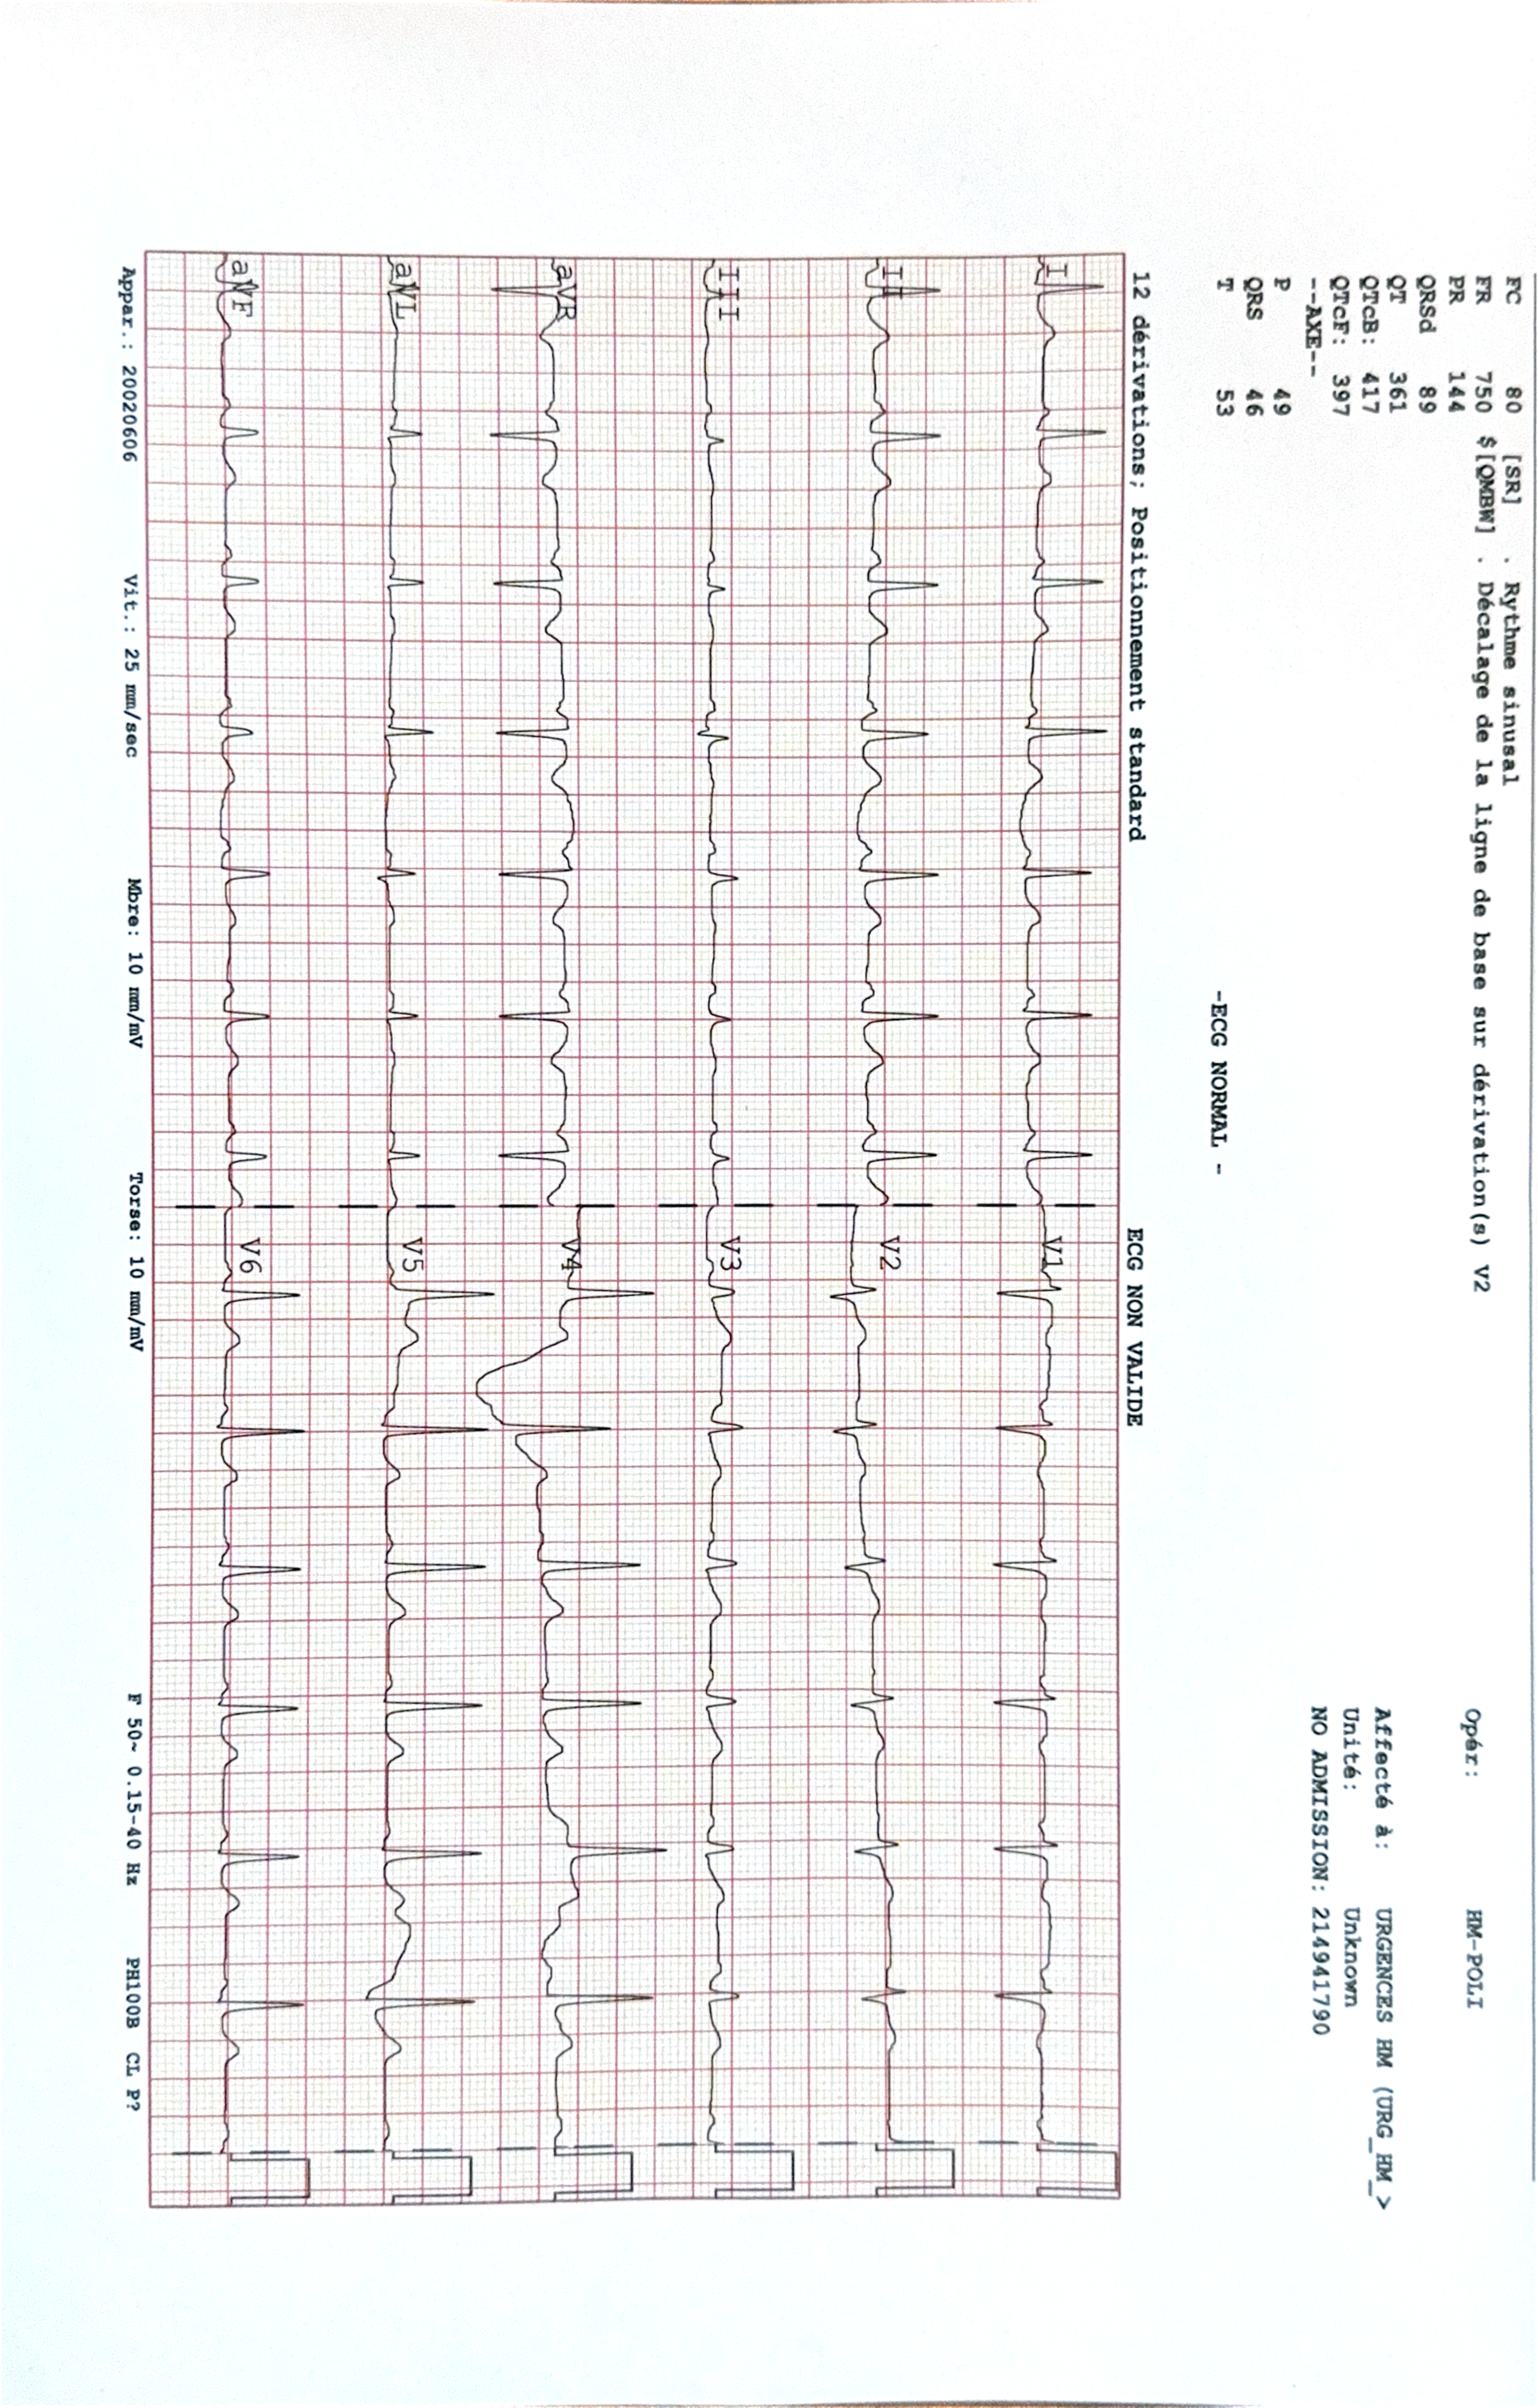
\includepdf[
  pages=1,
  scale=0.93,
  offset=0 0.35cm,
  pagecommand={%
    \thispagestyle{plain}%
    \phantomsection\label{annexe:examens_cas_m2}%
    \setAnnexBackLink{retour:examens_cas_iii}{Chap.\,III, \S~1.9}%
  }
]{figures/03-cas-therapeutique/ExamenParacliniqueCasM2.pdf}

% Page 2 d'ExamenParacliniqueCasM2.pdf : biologie CHL (1/2) du cas polypathologique (Chap. V, § 1.2)
\includepdf[
  pages=2,
  scale=0.93,
  offset=0 0.35cm,
  pagecommand={%
    \thispagestyle{plain}%
    \phantomsection\label{annexe:examens_cas_v}%
    \setAnnexBackLink{retour:examens_cas_v}{Chap.\,V, \S~1.2}%
  }
]{figures/03-cas-therapeutique/ExamenParacliniqueCasM2.pdf}

% Page 3 d'ExamenParacliniqueCasM2.pdf : biologie CHL (2/2) du cas polypathologique (Chap. V, § 1.2)
\includepdf[
  pages=3-,
  scale=0.93,
  offset=0 0.35cm,
  pagecommand={%
    \thispagestyle{plain}%
    \setAnnexBackLink{retour:examens_cas_v}{Chap.\,V, \S~1.2}%
  }
]{figures/03-cas-therapeutique/ExamenParacliniqueCasM2.pdf}

\clearpage
\thispagestyle{plain}
% Lien de retour préparé pour la 4e page (radioPatient.jpeg) : pointe actuellement vers le renvoi provisoire en fin de Chapitre VI et ne mène pas encore au bon endroit du Chapitre V
\setAnnexBackLink{retour:radio_patient}{Chap.\,VI, renvoi provisoire}
\phantomsection
\label{annexe:radio_patient}
\vspace*{\fill}
{\centering
  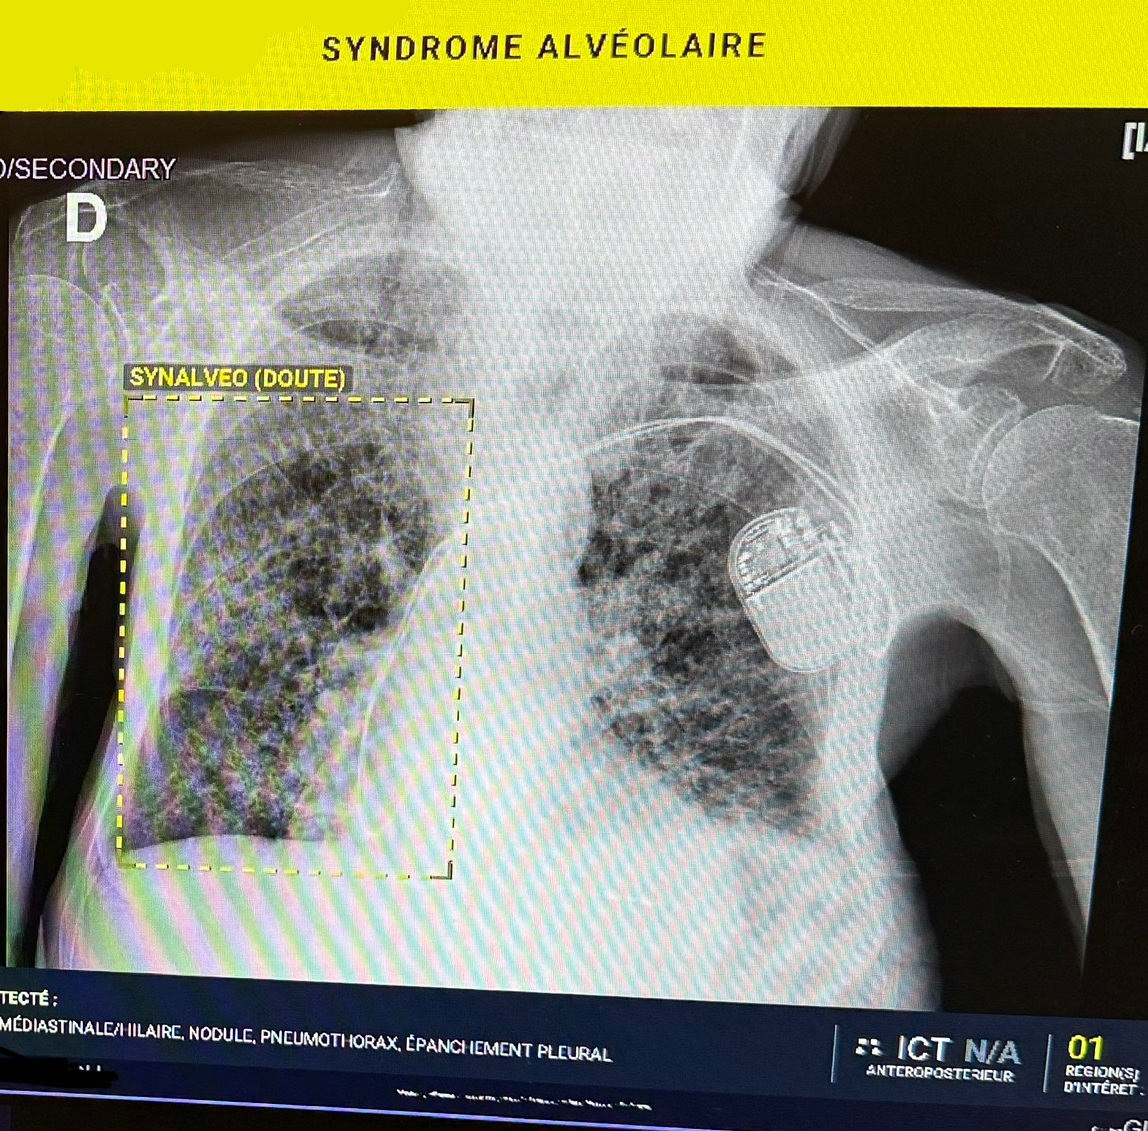
\includegraphics[width=\linewidth, height=0.86\textheight, keepaspectratio]{figures/05-cas-polypathologique-complexe/radioPatient.jpeg}\par}%
\todoH[GuillaumeVertStyle][green!25]{Lien de retour provisoire vers le Chap. VI : ne mène pas encore au bon endroit du Chap. V.}{}%
\vspace*{\fill}
\clearpage
\clearAnnexBackLink


\backmatter
\listoffigures
\listofillustrations
\listoftables
\printbibliography[title={Bibliographie}]

\end{document}
